%% 该模板修改自《计算机学报》latex 模板
%% 主要是将双栏改成单栏,去掉了部分计算机学报标识;
%% 源文件自:https://www.overleaf.com/latex/templates/latextemplet-cjc-xelatex/ybmmymncrrmw
%% 
%%
%% This is file `CjC_template_tex.tex',
%% is modified by Zhi Wang (zhiwang@ieee.org) based on the template 
%% provided by Chinese Journal of Computers (http://cjc.ict.ac.cn/).
%%
%% This version is capable with Overleaf (XeLaTeX).
%%
%% Update date: 2023/03/10
%% -------------------------------------------------------------------
%% Copyright (C) 2016--2023 
%% -------------------------------------------------------------------
%% This file may be distributed and/or modified under the
%% conditions of the LaTeX Project Public License, either version 1.3c
%% of this license or (at your option) any later version.
%% The latest version of this license is in
%%    https://www.latex-project.org/lppl.txt
%% and version 1.3c or later is part of all distribution`s of LaTeX
%% version 2008 or later.
%% -------------------------------------------------------------------

\documentclass[10.5pt,compsoc,UTF8]{CjC}
\usepackage{CTEX}
\usepackage{graphicx}
\usepackage{footmisc}
\usepackage{subfigure}
\usepackage{url}
\usepackage{multirow}
\usepackage{multicol}
\usepackage[noadjust]{cite}
\usepackage{amsmath,amsthm}
\usepackage{amssymb,amsfonts}
\usepackage{booktabs}
\usepackage{color}
\usepackage{ccaption}
\usepackage{booktabs}
\usepackage{float}
\usepackage{fancyhdr}
\usepackage{caption}
\usepackage{xcolor,stfloats}
\usepackage{comment}
\setcounter{page}{1}
\graphicspath{{figures/}}
\usepackage{cuted}%flushend,
\usepackage{captionhack}
\usepackage{epstopdf}
\usepackage{gbt7714}
\usepackage{listings}
\usepackage{xeCJK}
\usepackage{float}
\usepackage{sourcecodepro}
\usepackage[T1]{fontenc}
\usepackage{hyperref}

\setmainfont{Times Roman}
% \setCJKmainfont{Noto Sans Mono CJK TC}
\setCJKmainfont{標楷體.ttc}
\setmonofont{Cascadia Code}

%===============================%

\headevenname{\mbox{\quad} \hfill  \mbox{\zihao{-5}{ \hfill 2024 Hardware Design  } \hspace {50mm} \mbox{2024 年 10 月}}}%
\headoddname{Group 21 \hfill Lab 4: Finite State Machines}%

%footnote use of *
\renewcommand{\thefootnote}{\fnsymbol{footnote}}
\setcounter{footnote}{0}
\renewcommand\footnotelayout{\zihao{5-}}

\newtheoremstyle{mystyle}{0pt}{0pt}{\normalfont}{1em}{\bf}{}{1em}{}
\theoremstyle{mystyle}
\renewcommand\figurename{figure~}
\renewcommand{\thesubfigure}{(\alph{subfigure})}
\newcommand{\upcite}[1]{\textsuperscript{\cite{#1}}}
\renewcommand{\labelenumi}{(\arabic{enumi})}
\newcommand{\tabincell}[2]{\begin{tabular}{@{}#1@{}}#2\end{tabular}}
\newcommand{\abc}{\color{white}\vrule width 2pt}
\renewcommand{\bibsection}{}
\makeatletter
\renewcommand{\@biblabel}[1]{[#1]\hfill}
\makeatother
\setlength\parindent{2em}
%\renewcommand{\hth}{\begin{CJK*}{UTF8}{gbsn}}
%\renewcommand{\htss}{\begin{CJK*}{UTF8}{gbsn}}
\renewcommand{\contentsname}{Table of Contents}

\begin{document}

\hyphenpenalty=50000
\makeatletter
\newcommand\mysmall{\@setfontsize\mysmall{7}{9.5}}
\newenvironment{tablehere}
  {\def\@captype{table}}

\let\temp\footnote
\renewcommand \footnote[1]{\temp{\zihao{-5}#1}}

\hypersetup{
  colorlinks=false,
  pdfborder={0 0 0},
}

\thispagestyle{plain}%
\thispagestyle{empty}%
\pagestyle{CjCheadings}

% \begin{table*}[!t]
\vspace {-13mm}


\onecolumn
\zihao{5-}\noindent Group 21 \hfill Lab 4: Finite State Machines \hfill 2024 年 10 月\\
\noindent\rule[0.25\baselineskip]{\textwidth}{1pt}


\begin{center}
    \vspace {11mm}
    {\zihao{2} \heiti \fangsong Lab 4: Finite State Machines }
    
    \vskip 5mm
    
    {\zihao{4}\fangsong Group 21: 陳克盈(112062205)、蔡明妡(112062224)}
\end{center}

\lstset{
    % backgroundcolor=\color{red!50!green!50!blue!50},%程式碼塊背景色為淺灰色
    rulesepcolor= \color{gray}, %程式碼塊邊框顏色
    breaklines=true,  %程式碼過長則換行
    numbers=left, %行號在左側顯示
    numberstyle= \small\ttfamily,%行號字型
    keywordstyle= \color{blue},%關鍵字顏色
    commentstyle=\color{gray}, %註釋顏色
    frame=shadowbox%用方框框住程式碼塊
    basicstyle=\ttfamily\footnotesize,
}
 
\definecolor{improvecolor}{rgb}{0,0.6,0} % 深綠色
\definecolor{declinecolor}{rgb}{0.6,0,0} % 深紅色


%%%%%%%%%%%%%%%%%%%%%%%%%%%%%%%%%%%%%%
\zihao{5}
\vskip 10mm
% \begin{multicols}{1}


%%%%%%%%%%%%%%%%%%%%%%%%%%%%%%%%%%%%%%%%%%
%%%%%%%%%%%%%%%%%%%%%%%%%%%%%%%%%%%%%%%%%%

\tableofcontents
\newpage

\section{Basic Question: LFSR}
Linear-Feedback Shift Register (LFSR),是一種透過種子(初始值)來生成一系列數字序列的偽隨機產生器。\
LFSR 會透過狀態內數值的互相 XOR,達到產生新隨機值的效果。又可根據內部架構的不同,分為 Many-to-one LFSR 與 One-to-many LFSR。

\begin{itemize}
  \item Many-to-one LFSR: 以 Basic Question 的架構為例,下一個狀態的 $DFF[0]$ 會受到前一個狀態中,\\
  $DFF[1], DFF[2], DFF[3], DFF[7]$ 互相 XOR 後的值影響。\
  因為是多個 bit 影響一個 bit,所以稱為 Many-to-one LFSR。
  \item One-to-many LFSR: 同樣以 Basic Question 的架構為例,下一個狀態的 $DFF[2], DFF[3], DFF[4]$ 會分別受到上個狀態中,\
  其前一位與 $DFF[7]$ XOR 後的值影響。因為是一個 bit 影響多個 bit,所以稱為 One-to-many LFSR。
\end{itemize}

這兩種架構都有一個共通點,就是一開始的種子不能全為 0,否則就會因為 $0 \oplus 0 = 0$ 的特性,導致輸出值永遠都不會改變。

\section{Q1: Content-addressable memory (CAM)}

\begin{itemize}
  \item input clk: clock
  \item input wen: write enable
  \item input ren: read enable
  \item input [3:0] addr: address
  \item output [3:0] dout: output data
  \item output hit: hit signal
\end{itemize}

這題需要我們用 16 個 8-bit 組成的 data line,實作出一個 Content Addressable Memory (CAM)。\
基本操作有兩種:

\begin{itemize}
  \item Read: 當 read enable 訊號為 1 時,找到在記憶體中,與 $din$ 一樣的記憶體位址,並將其輸出到 $dout$,並將 $hit$ 設定為 $1$。\
  如果有多個記憶體位置的值與 $din$ 一樣,則輸出最大的位址。若記憶體中沒有對應的資料,則輸出 $0$ 並將 hit 設定為 $0$。
  \item Write: 當 write enable 訊號為 1 且 read enable 訊號為 0 時,將 $din$ 寫入到記憶體中的 $addr$ 位址。
\end{itemize}

\subsection{Implement}
整體架構主要由三個部分組成:Stored data line, Comparator Array, Priority Encoder。

\subsubsection*{Stored data line}
每個 Data line 用 8 個 DFF 來儲存資料,共有 16 個 Data line。
\par
當要寫入時,會直接將資料寫入至第 $addr$ 個 Data line。\
而讀取時則是會將 $16$ 筆資料輸入至下個部分的 Comparator Array。
\par
由於 DFF 在初始化前會是 X,所以在判斷是否有 hit 的時候,使用 === 運算子來避免 X 對於 hit 的影響。

\subsubsection*{Comparator Array}
這部分會直接將 $16$ 筆資料中,enable bit 為 1 的位址與 $din$ 進行比較,並將 $16$ 個比較結果輸入至 Priority Encoder。\
下圖是一個單位的 Comparator Array,實際應用時會有 16 個這樣的單位,用來比較所有的 Data line

\begin{figure}[h!]
  \centering
  
\includegraphics[width=0.8\textwidth]{./img/Q1-CA.png}
  \caption{Comparator Array}
  \label{fig:CA}
\end{figure}

\newpage
\subsubsection*{Priority Encoder}
這部分再程式碼的實作上,會從第 $15$ 個 Data line 開始,找到第一個比較結果為 1 的位址,並將其輸出至 $dout$。\
不過因為電路上是越靠近輸出的優先序越高,因此畫成電路後,會從第 $0$ 個 Data line 開始比較。

\begin{figure}[h!]
  \centering
  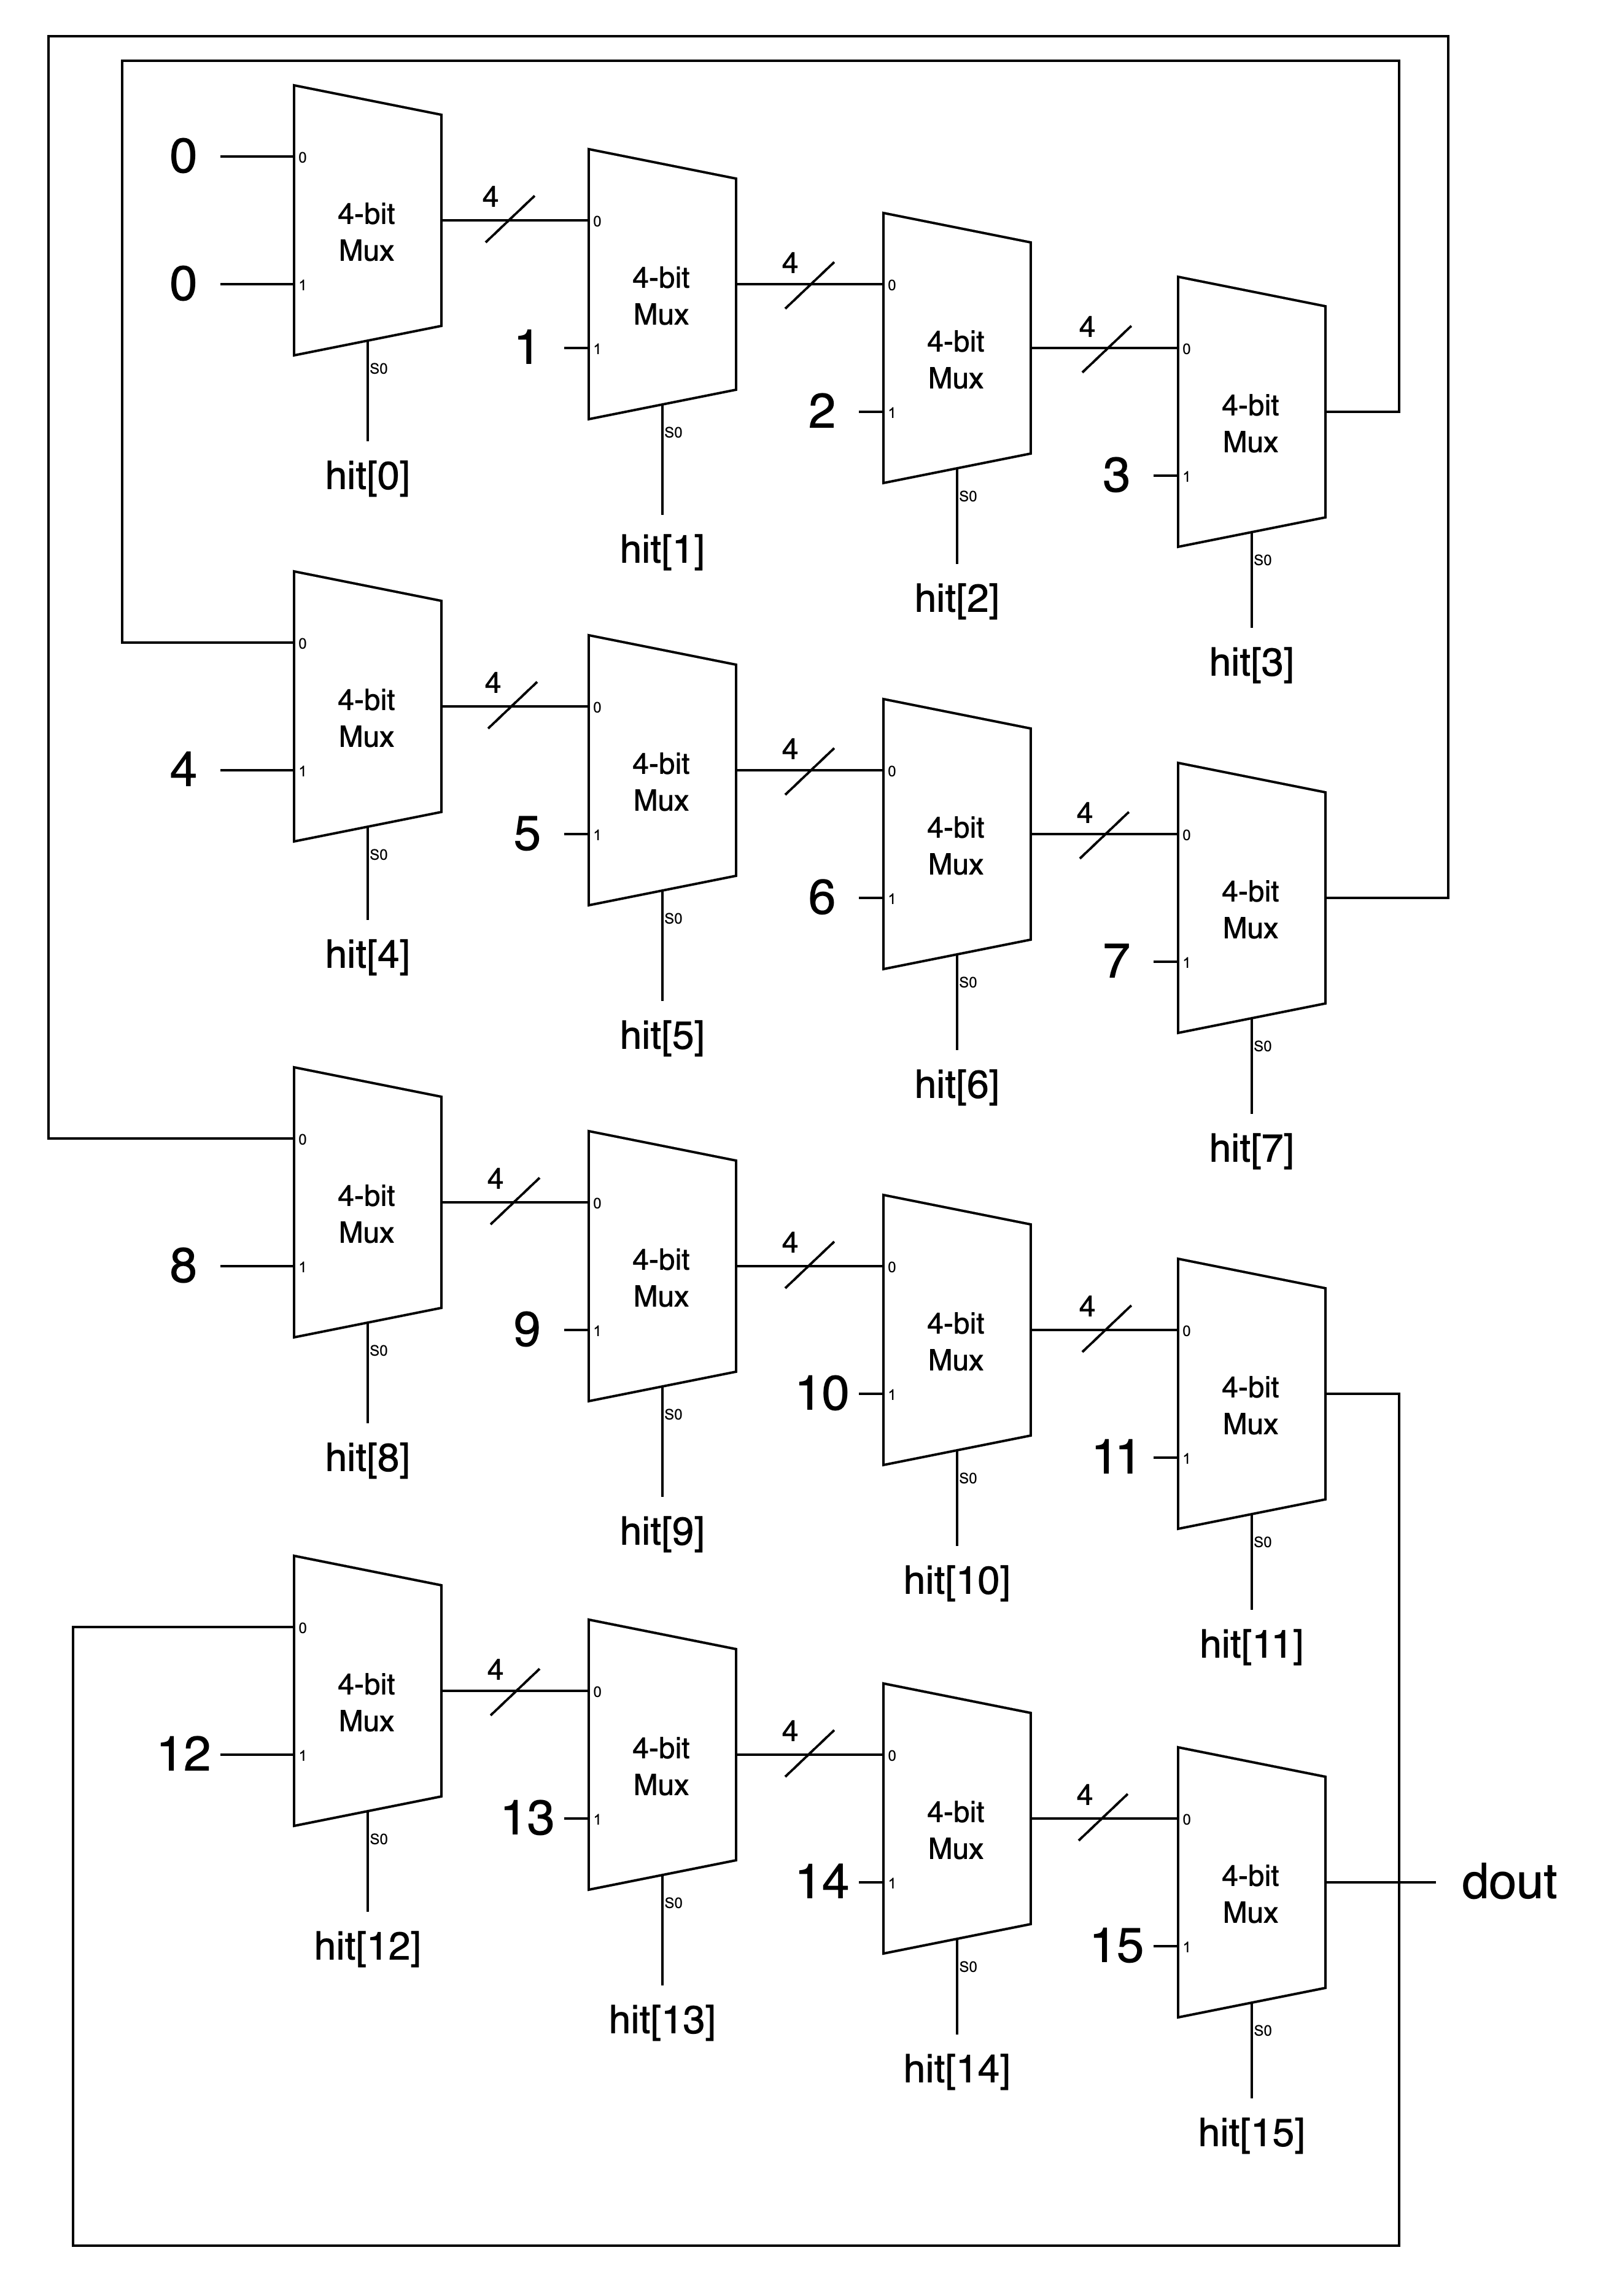
\includegraphics[width=0.8\textwidth]{./img/Q1-PE.png}
  \caption{Priority Encoder}
  \label{fig:PE}
\end{figure}
\newpage

\subsubsection*{Overall}

將三個部分組合在一起,架構就會如下圖所示:
\begin{figure}[h!]
  \centering
  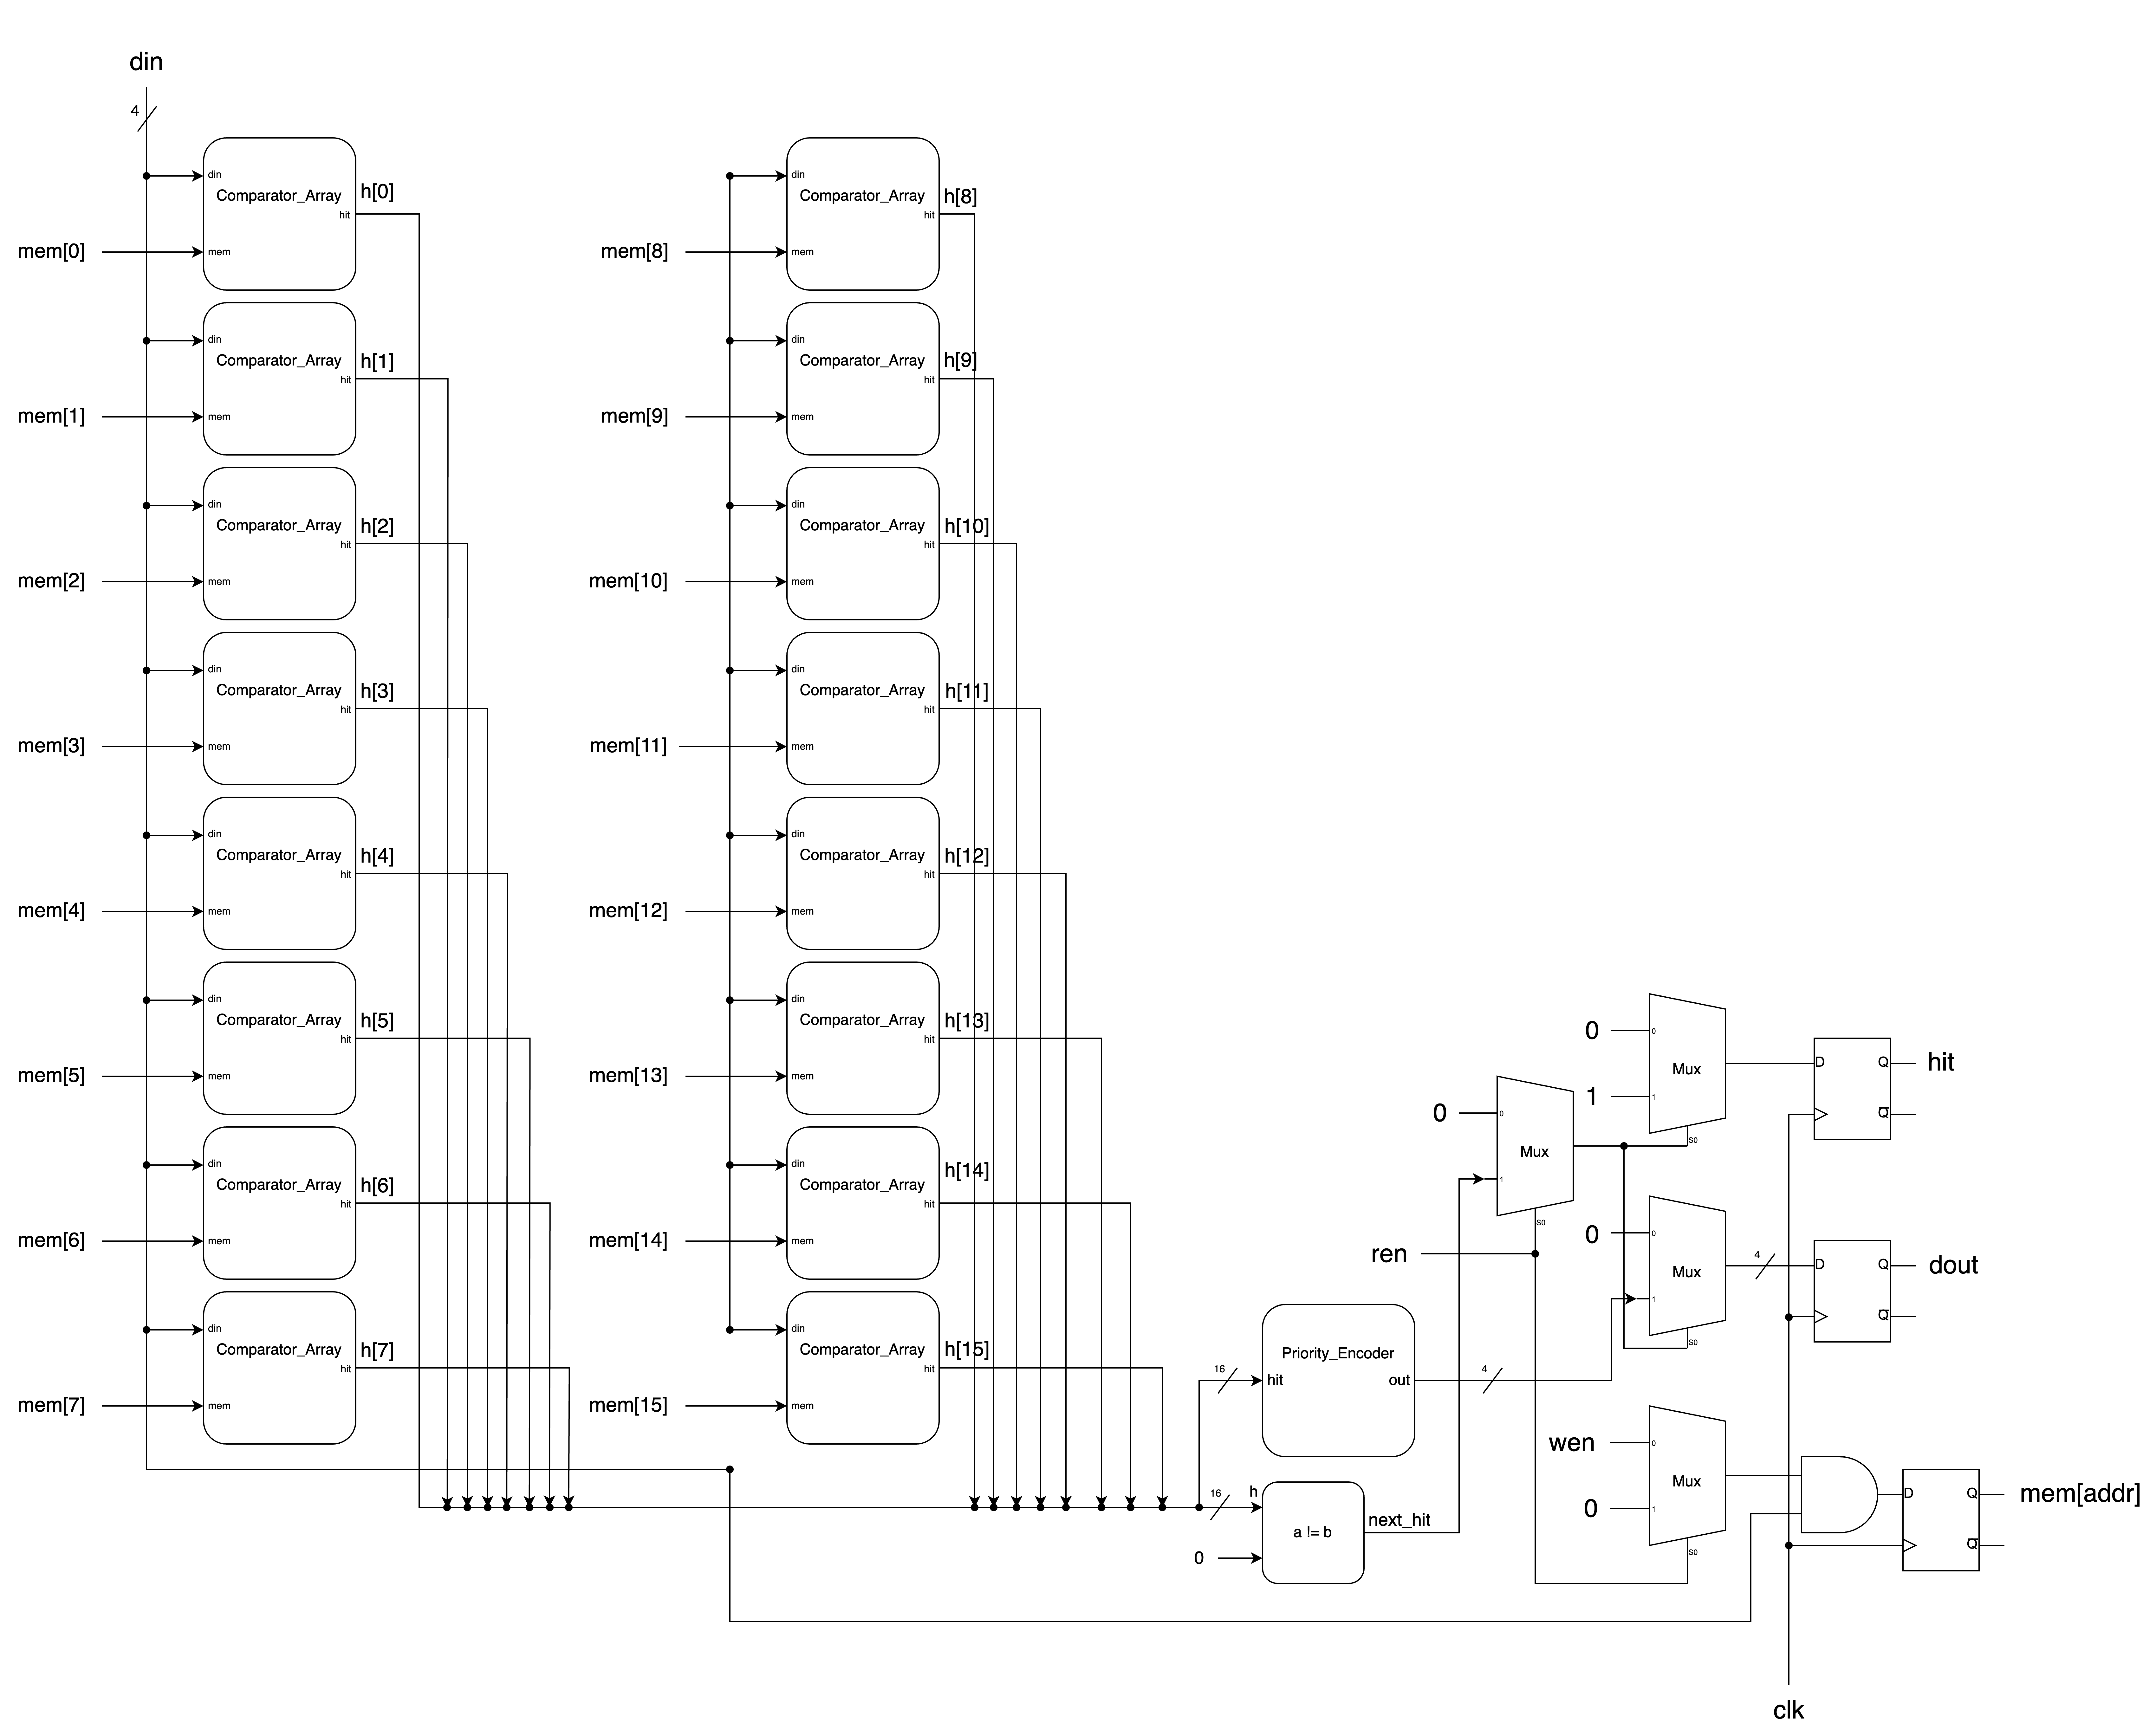
\includegraphics[width=\textwidth]{./img/Q1.png}
  \caption{Q1 Overall}
  \label{fig:Q1-Overall}
\end{figure}
\newpage

\subsection{Testbench}
\begin{figure}[h!]
  \centering
  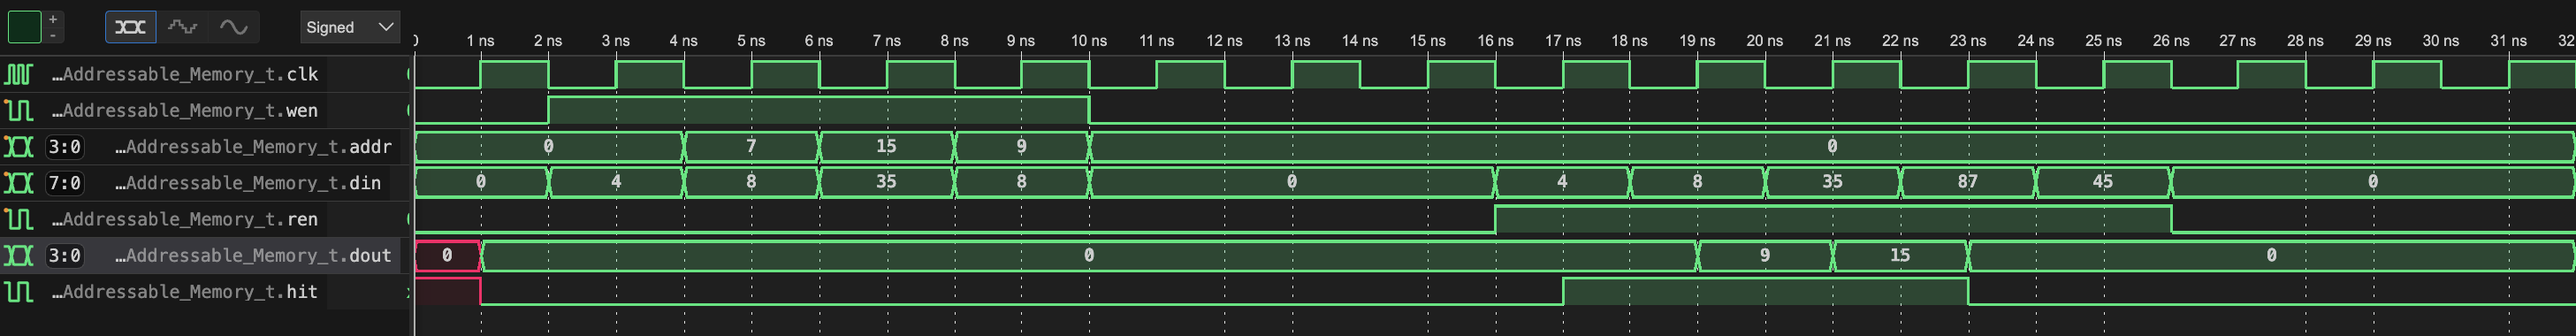
\includegraphics[width=\textwidth]{./img/Q1-tb.png}
  \caption{Q1 Testbench}
  \label{fig:Q1-tb}
\end{figure}

\section{Q2: Scan chain design}
\begin{itemize}
  \item input clk: clock
  \item input rst\_n: not reset
  \item input scan\_in: scan input
  \item input scan\_en: scan enable
  \item output scan\_out: scan output
\end{itemize}

這題要實作一個用來測試 4-bit 乘法器的 Scan chain,由一個 4-bit 乘法器以及 8 個 Scan-DFF 組成,\
執行時會有三種階段(操作):
\begin{enumerate}
  \item Scan in: 當 $scan\_en$ 為 1 時,SDFF 的資料會右移一位,空出來的 $SDFF[7]$(最左側的 SDFF)則會接收 $scan\_in$ 的值。\
  這個階段若經過了 8 個 clock cycle,就能夠將要放入乘法器的兩筆 4-bit 資料 $a, b$ 讀入 SDFF 中。
  \item Capture: 當 $scan\_en$ 為 0 時,SDFF 會停止接收資料,並將 $SDFF[7:4]$ 作為 $a$, \
  $SDFF[3:0]$ 作為 $b$,傳入乘法器中進行運算。經過了一個 clock 後,乘法器的結果就會被寫入至 SDFF 中。
  \item Scan out: 呼應 Scan in 階段,當 $scan\_en$ 為 1 時,SDFF 的資料會右移一位,\
  被 pop 出來的 $SDFF[0]$ 就會作為 $scan\_out$ 被輸出出來。此階段若經過了 $8$ 個 clock cycle,\
  就會將前一個階段的乘法器結果,以 $p[0], p[1], \dots, p[7]$ 的順序全部輸出出來。
\end{enumerate}

直得注意的是,Scan in 與 Scan out 是可以同步進行的,也就是說,當 $scan\_en = 1$ 時,\
SDFF 們會接收 $scan\_in$,並將舊的資料輸出至 $scan\_out$。

\subsection{Implement}

\subsubsection*{SDFF}
首先介紹 Scan-DFF,這是基於基礎的 DFF 加上兩個 MUX得來。\
第一個 MUX 利用 $scan\_en$ 控制資料輸入來源為 $scan\_in\ (scan\_en = 1)$ 或是乘法器 $(scan\_en = 0)$,\
另一個則是利用 $rst\_n$ 控制 DFF 是要接收上一個 MUX 的輸出結果 $(rst\_n = 1)$,還是初始化為 0 $(rst\_n = 0)$

\begin{figure}[h!]
  \centering
  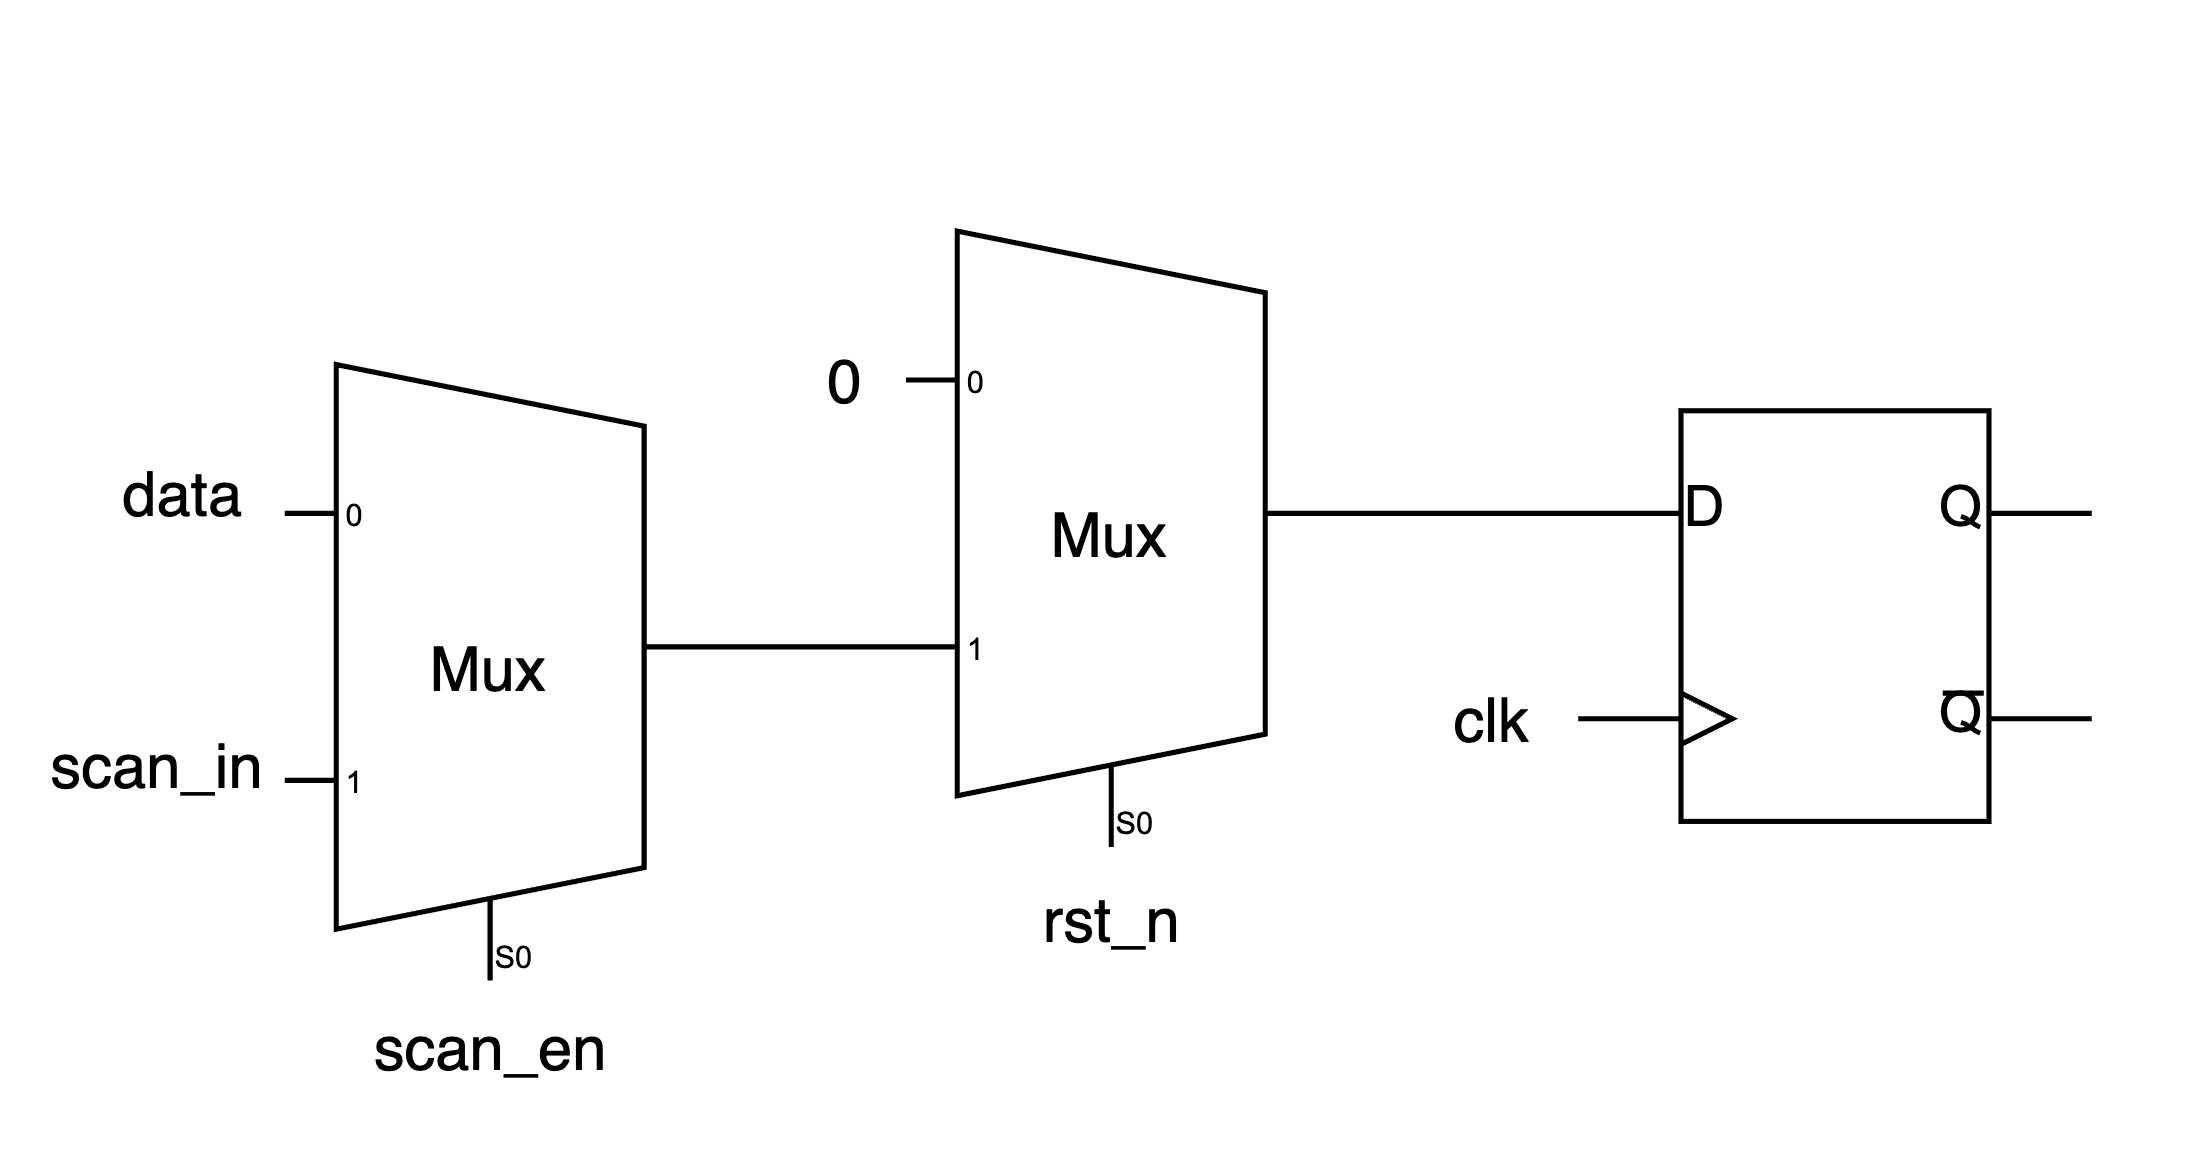
\includegraphics[width=0.8\textwidth]{./img/Q2-SDFF.png}
  \caption{Scan-DFF}
  \label{fig:SDFF}
\end{figure}

\subsubsection*{Overall}
接著將 8 個 SDFF 以及 4-bit 乘法器組合在一起,SDFF 的輸出將會被作為乘法器以及下一個 SDFF 的輸入,\
而乘法器的輸出則會作為 SDFF 的 $data$ 輸入。\
\par
用這樣的方式,電路就會在 $scan\_en$ 為 True 的時候從 $scan\_in$ 讀入資料,\
並在 $scan\_en$ 為 False 的時候將乘法器的結果紀錄至 SDFF。

\begin{figure}[h!]
  \centering
  
\includegraphics[width=\textwidth]{./img/Q2.png}
  \caption{Q2 Overall}
  \label{fig:Q2-Overall}
\end{figure}
\newpage
\subsection{Testbench}
這邊展示了 $5 \times 5 = 25$ 的例子:

\begin{figure}[h!]
  \centering
  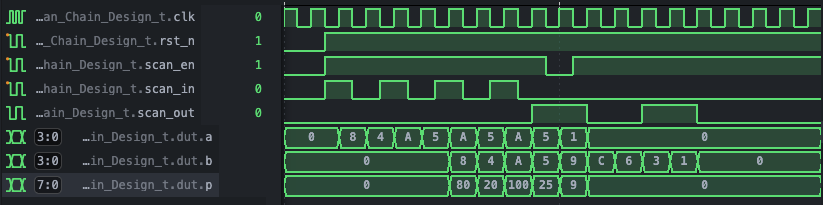
\includegraphics[width=\textwidth]{./img/Q2-tb.png}
  \caption{Q2 Testbench}
  \label{fig:Q2-Testbench}
\end{figure}


\section{Q3: Built-in self test (BIST)}
\begin{itemize}
  \item input clk: clock
  \item input rst\_n: not reset
  \item input scan\_en: scan enable
  \item output scan\_in: scan input
  \item output scan\_out: scan output
\end{itemize}

既然我們已經在 Basic 中實作了一個偽隨機產生器,那麼我們就能夠將其運用在 Scan chain 的測試中。\
而這也是這題的要求,我們需要將 LFSR 產生的偽隨機序列,作為 Scan chain 的輸入,實現一個 Built-in self test (BIST)。
\newpage
\subsection{Implement}
將 Basic 中實現的 Many-to-one LFSR 作為 BIST 的輸入,並將其輸出接至 Scan chain 的 $scan\_in$ 即可。

\begin{figure}[h!]
  \centering
  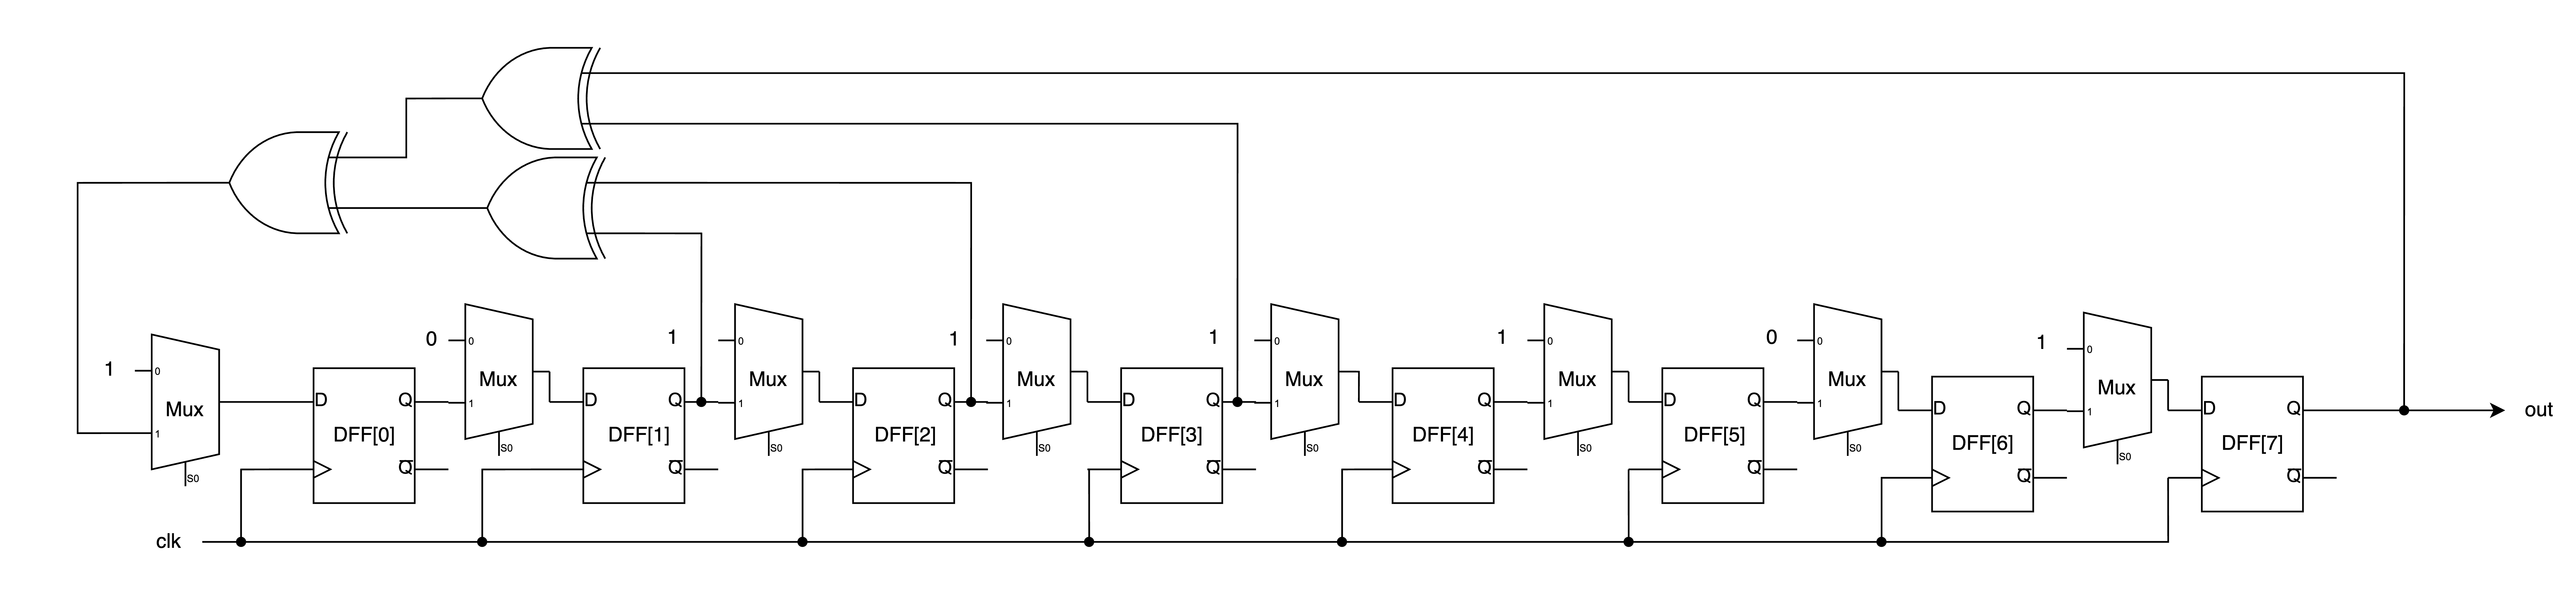
\includegraphics[width=\textwidth]{./img/Q3-LFSR.png}
  \caption{LFSR}
  \label{fig:LFSR}
\end{figure}

\begin{figure}[h!]
  \centering
  
\includegraphics[width=0.8\textwidth]{./img/Q3.png}
  \caption{Q3 Overall}
  \label{fig:Q3-Overall}
\end{figure}

\section{Q4: Mealy machine sequence detector}
\begin{itemize}
  \item input clk: clock
  \item input rst\_n: not reset
  \item input In: input
  \item output Dec: output
\end{itemize}

這題要實作一個 Mealy machine,用來偵測輸入是不是 $0111, 1001, 1110$ 這三個序列中的其中一個。\
且每四個 Bit 就要重新偵測。也就是說,在偵測到地 4 個 bit 後,如果符合其中一個序列,就會輸出 $1$,否則輸出 $0$。

\subsection{State Diagram}

我們需要先畫出 Mealy machine 的狀態圖。首先,我們先將 $0111, 1001, 1110$ 這三種序列的狀態圖給畫出來,\
如下圖所示,紅色代表 $1110$,綠色代表 $0111$,藍色代表 $1001$。

\begin{figure}[h!]
  \centering
  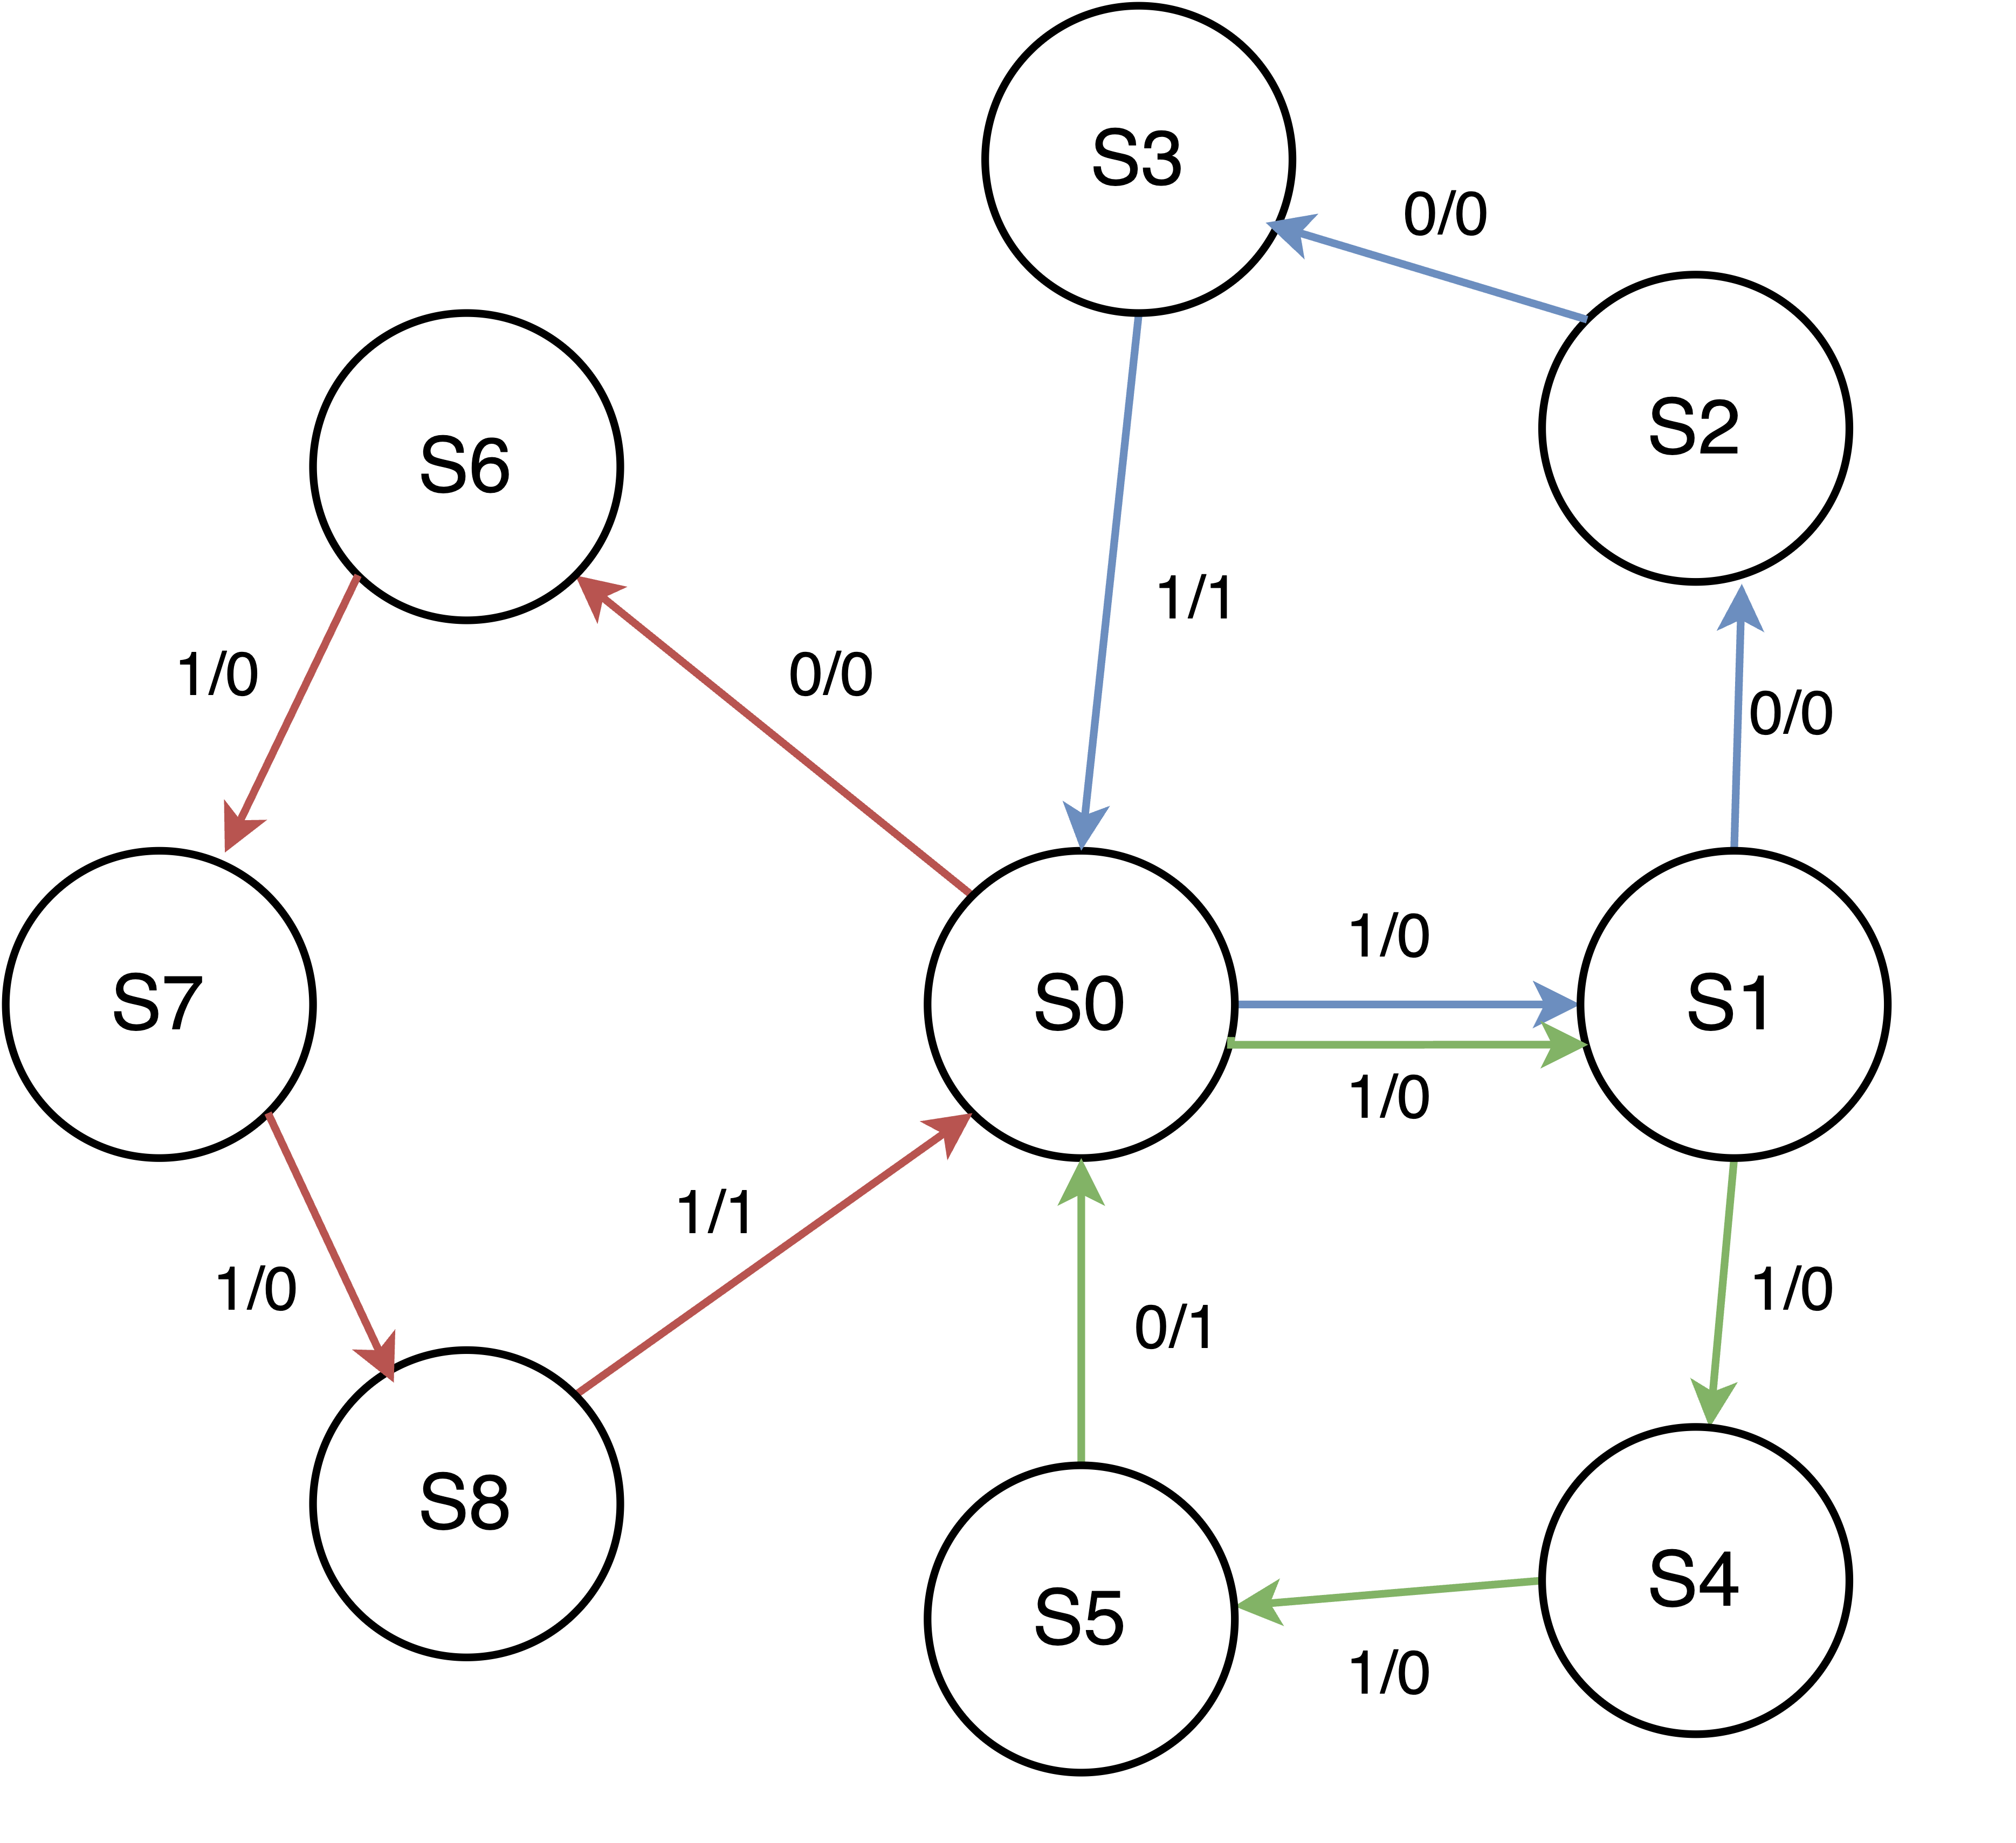
\includegraphics[width=0.4\textwidth]{./img/Q4-SD1.png}
  \caption{Step 1}
  \label{fig:SD1}
\end{figure}

接著,我們可以發現,State 3 與 State 8 一樣,都是當輸入為 1 時,輸出 1 並進到狀態 0。\
因此我們可以將這兩個狀態合併:

\begin{figure}[h!]
  \centering
  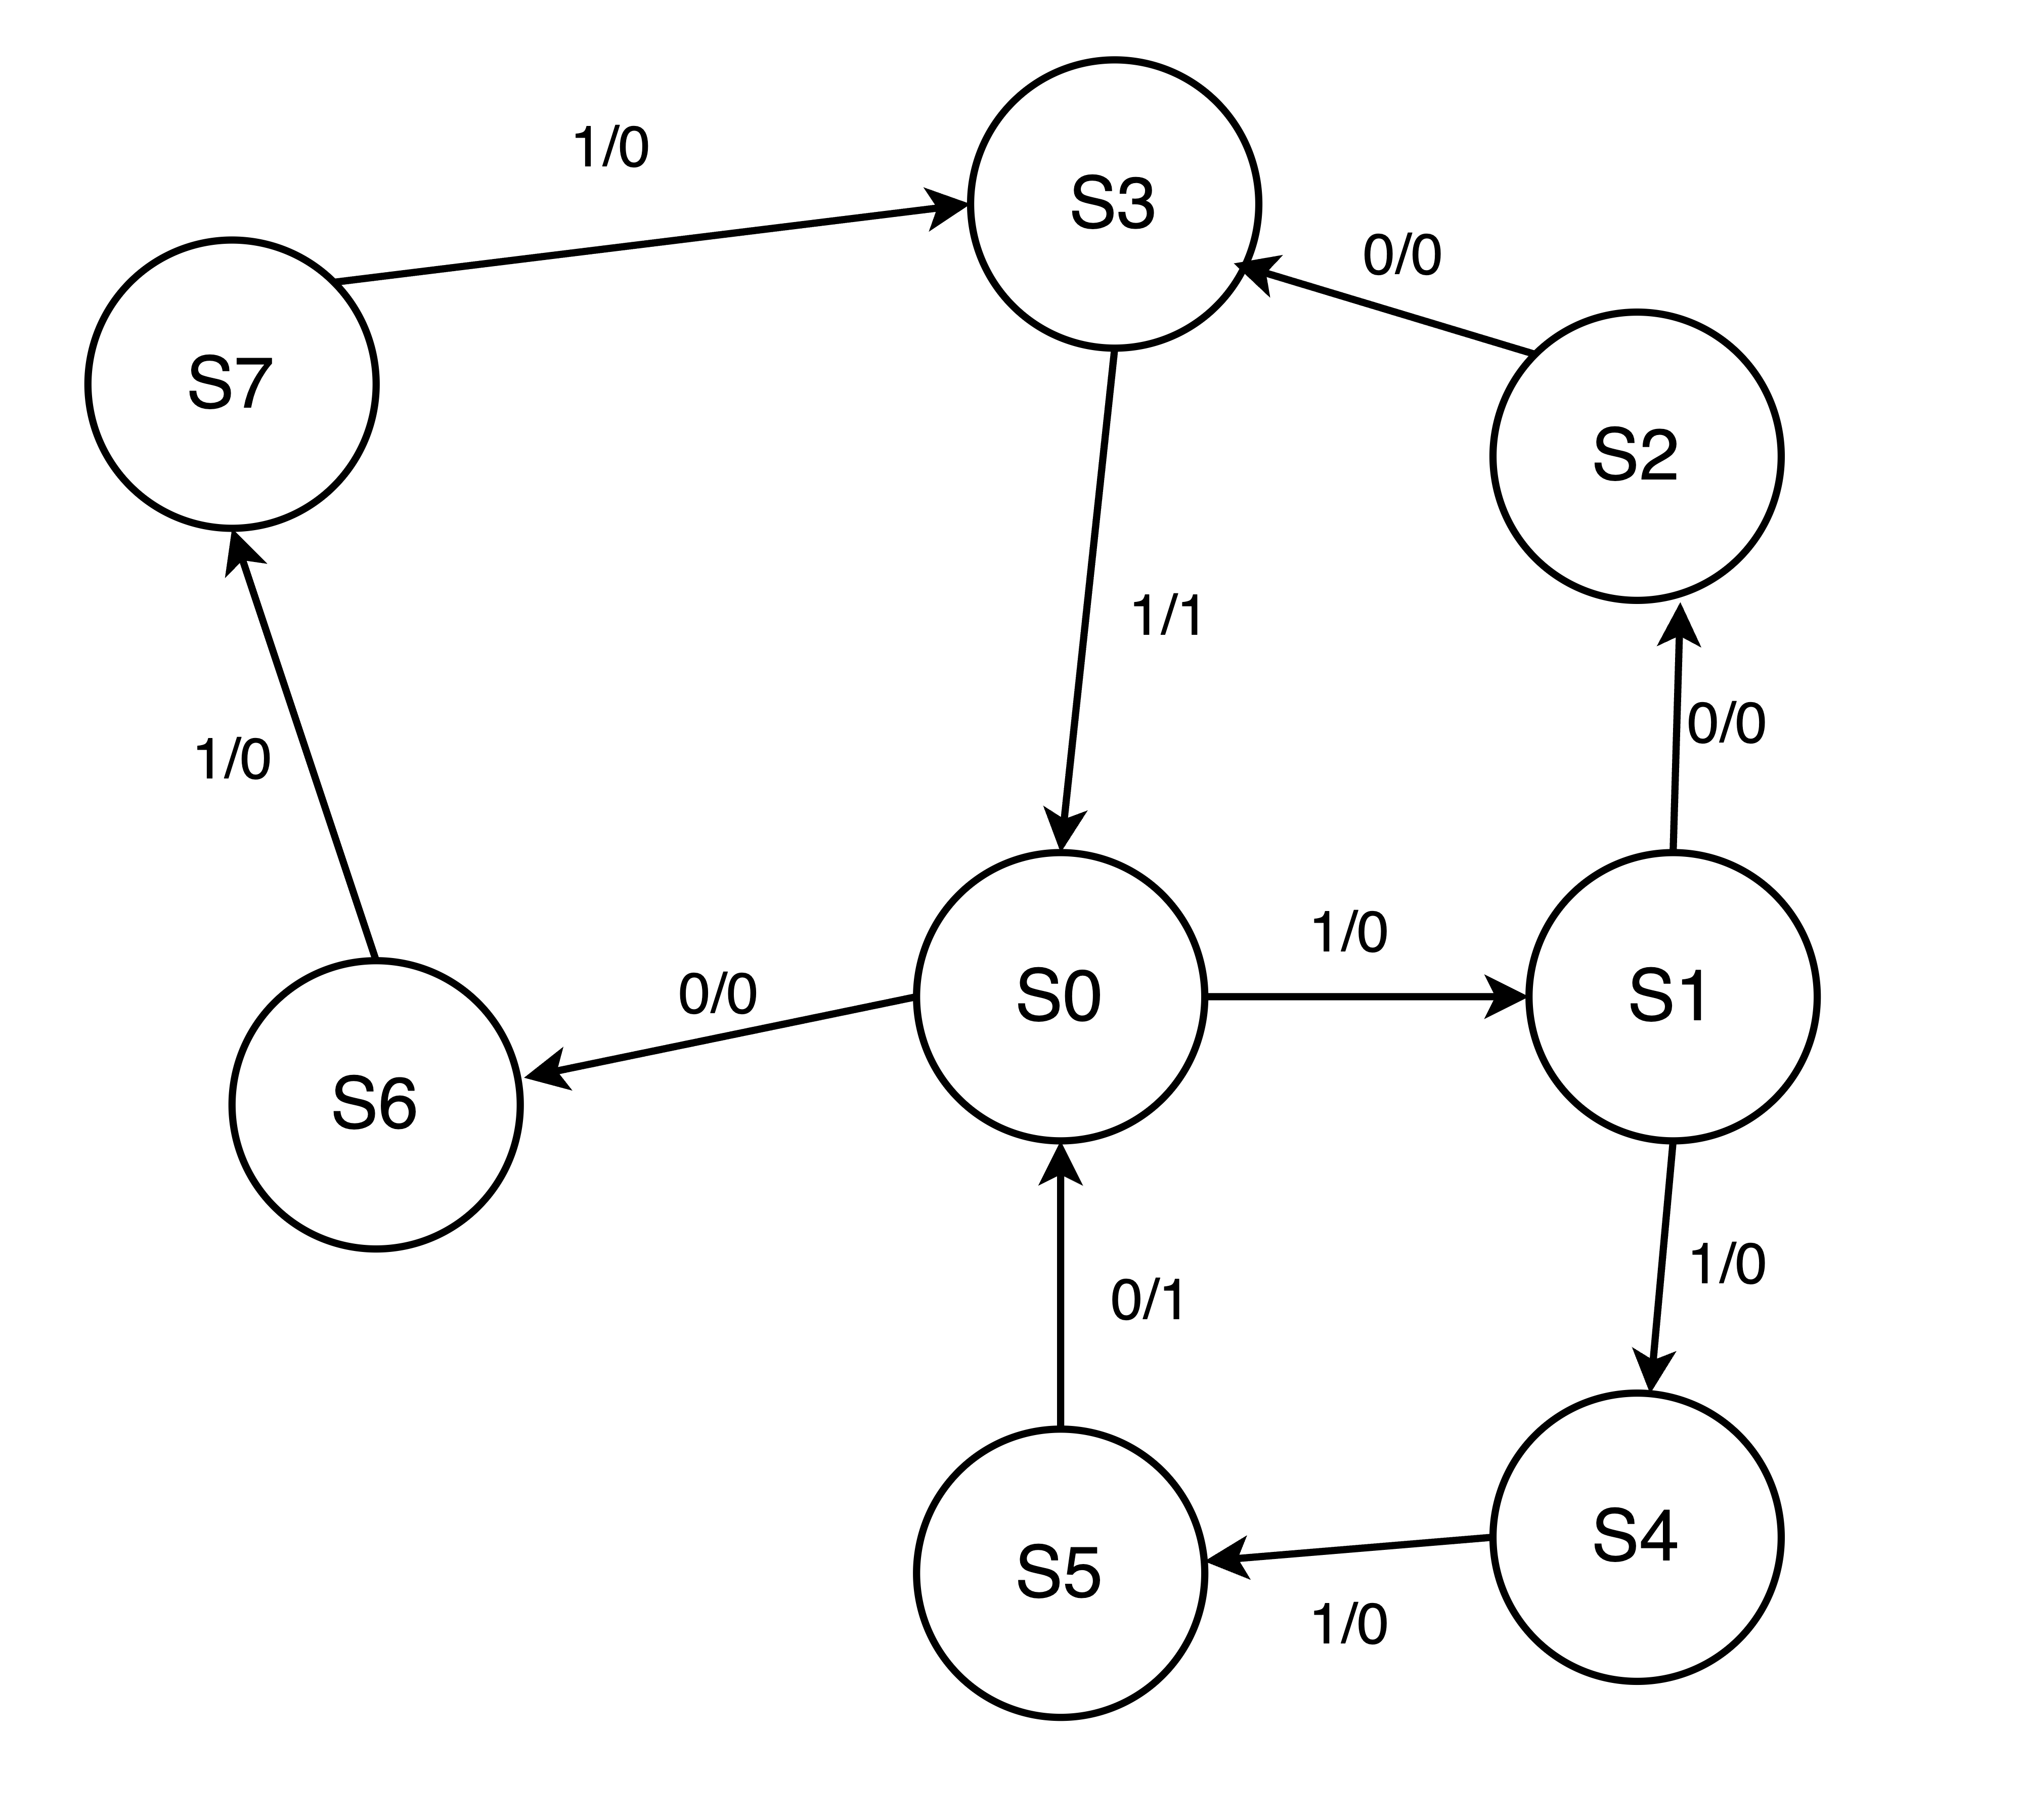
\includegraphics[width=0.4\textwidth]{./img/Q4-SD2.png}
  \caption{Step 2}
  \label{fig:SD2}
\end{figure}

\newpage
最後,由於剩下的可能全都不是我們要的,因此將沒畫到的可能全部都指向 State 0 並輸出 0 即可。

\begin{figure}[h!]
  \centering
  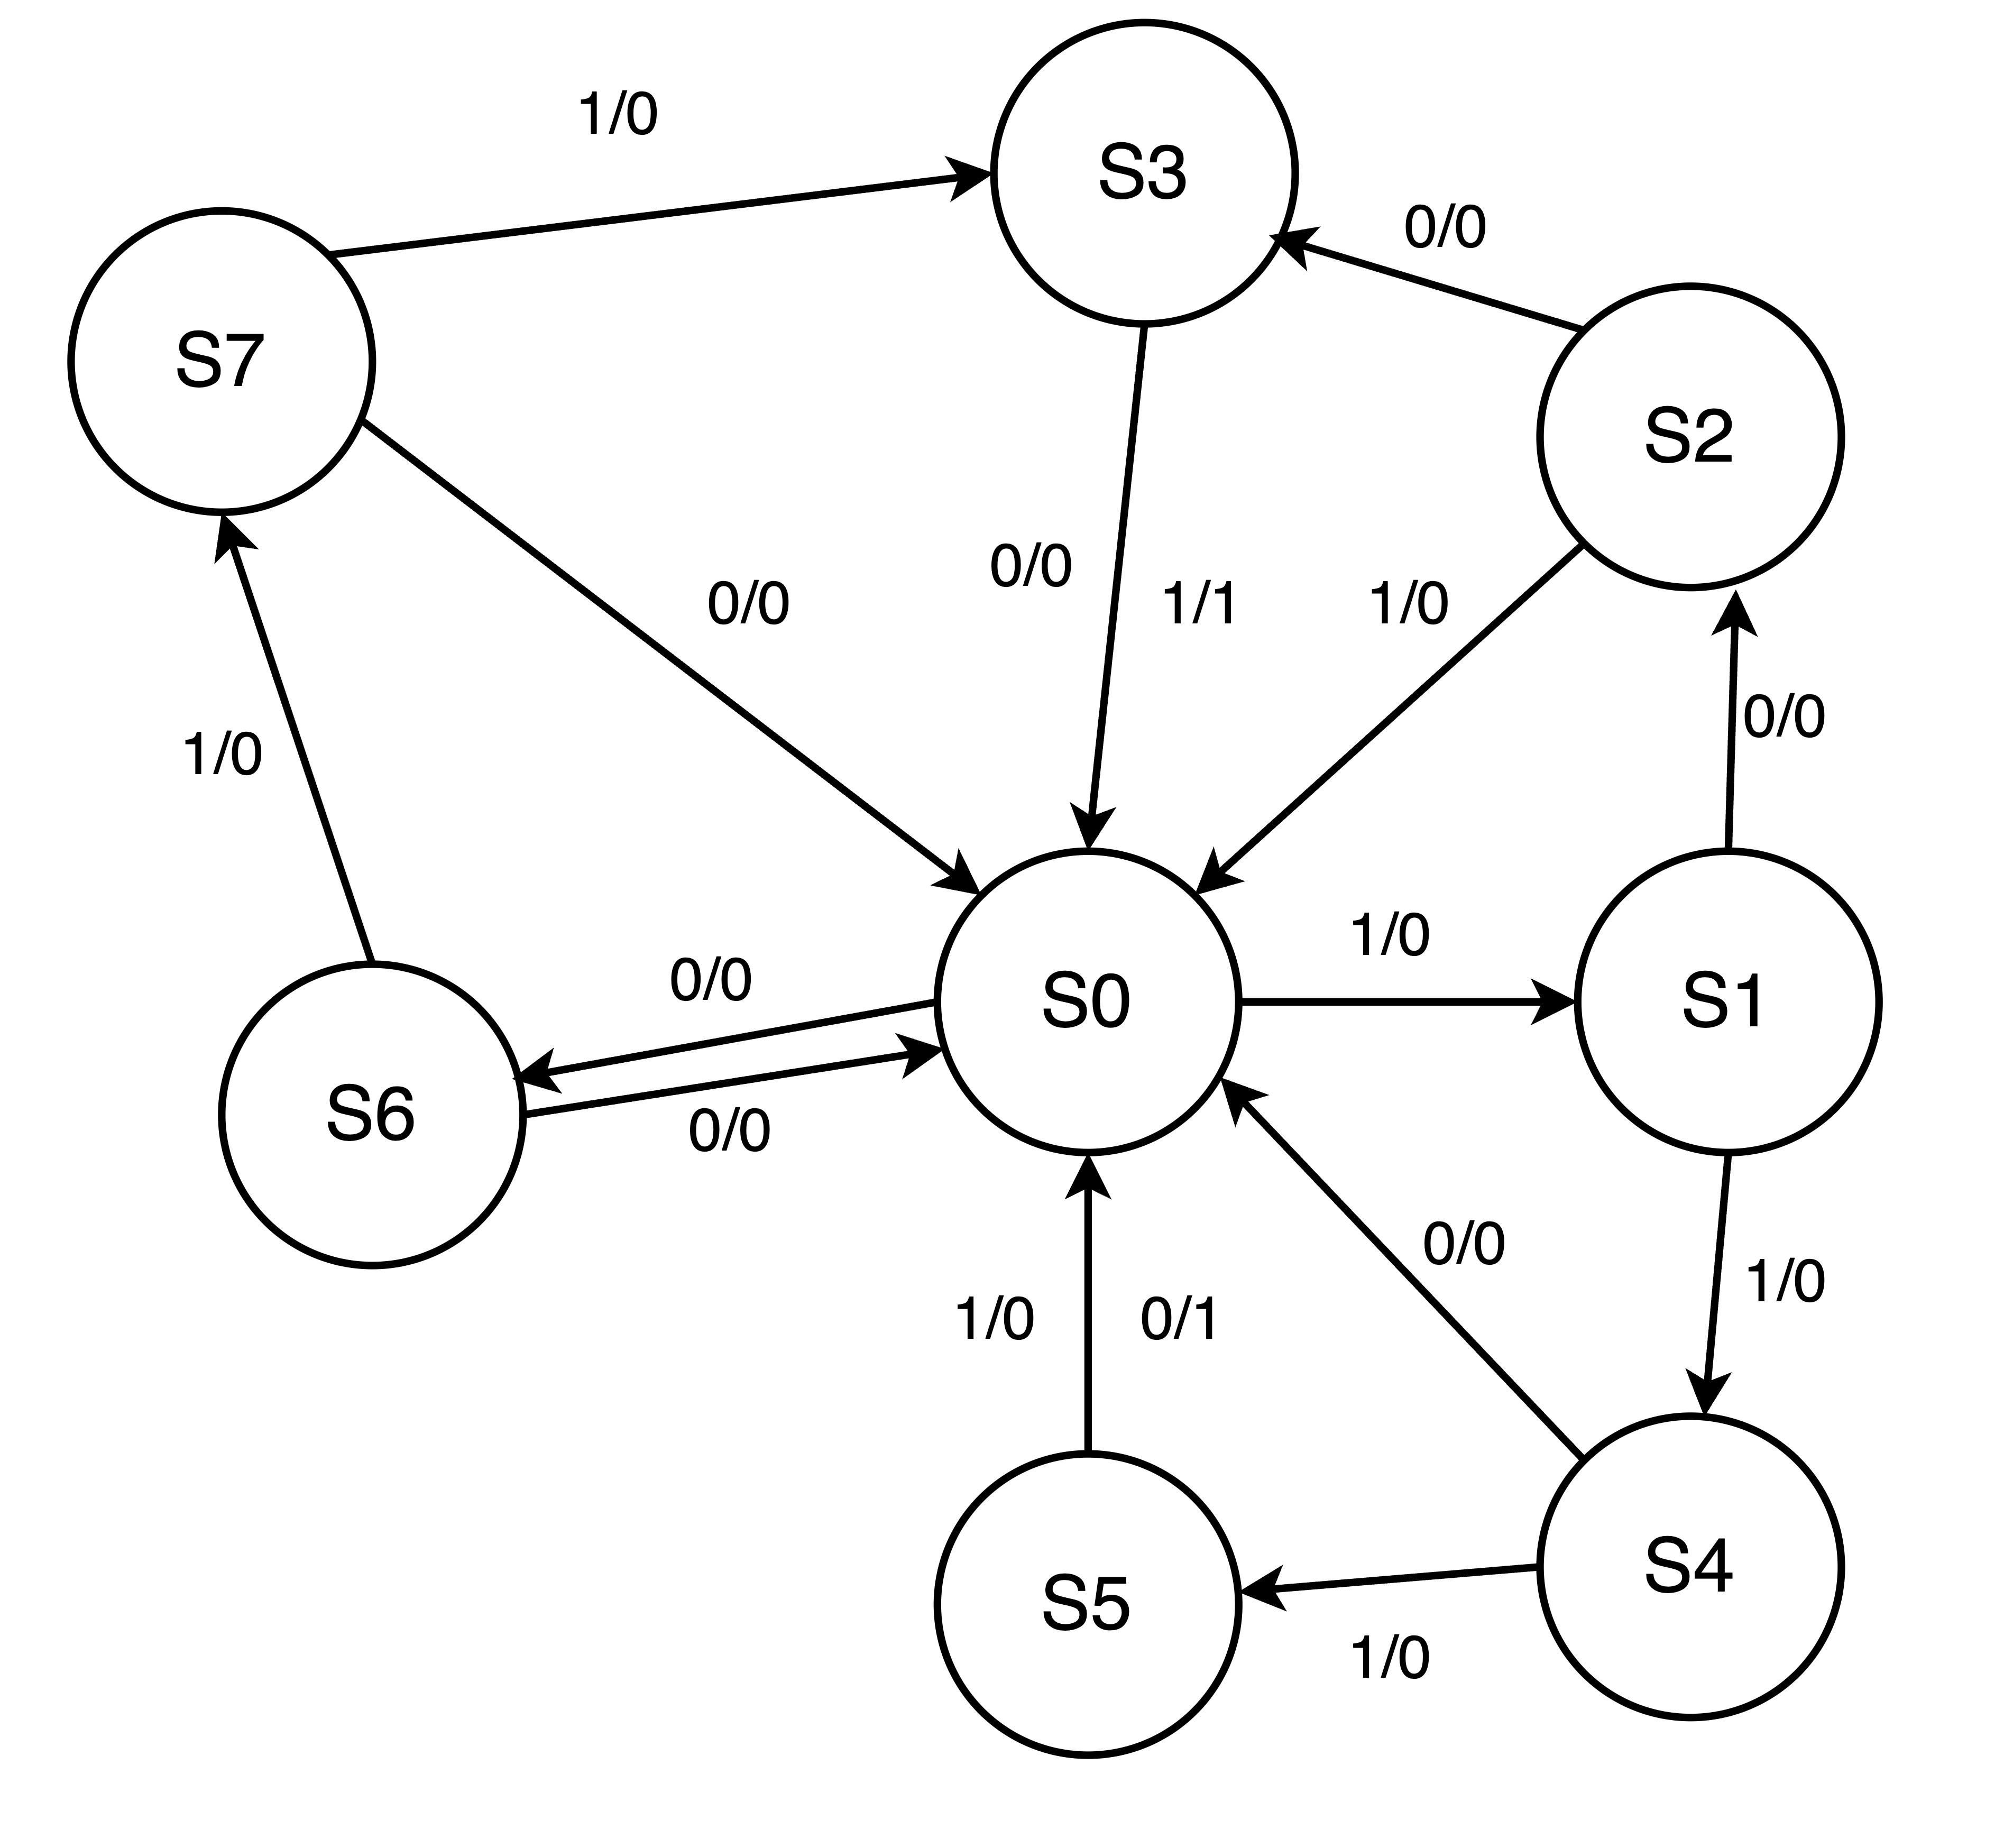
\includegraphics[width=0.4\textwidth]{./img/Q4-SD3.png}
  \caption{Step 3}
  \label{fig:SD3}
\end{figure}

\newpage
\subsection{Implement}

在實作上還有一個細節要注意,因為每 4 個 bit 需要重置狀態,因此我們額外使用了一個 counter,每次 counter 數到第四個的時候,\
就強制回到 State 0。

\begin{figure}[h!]
  \centering
  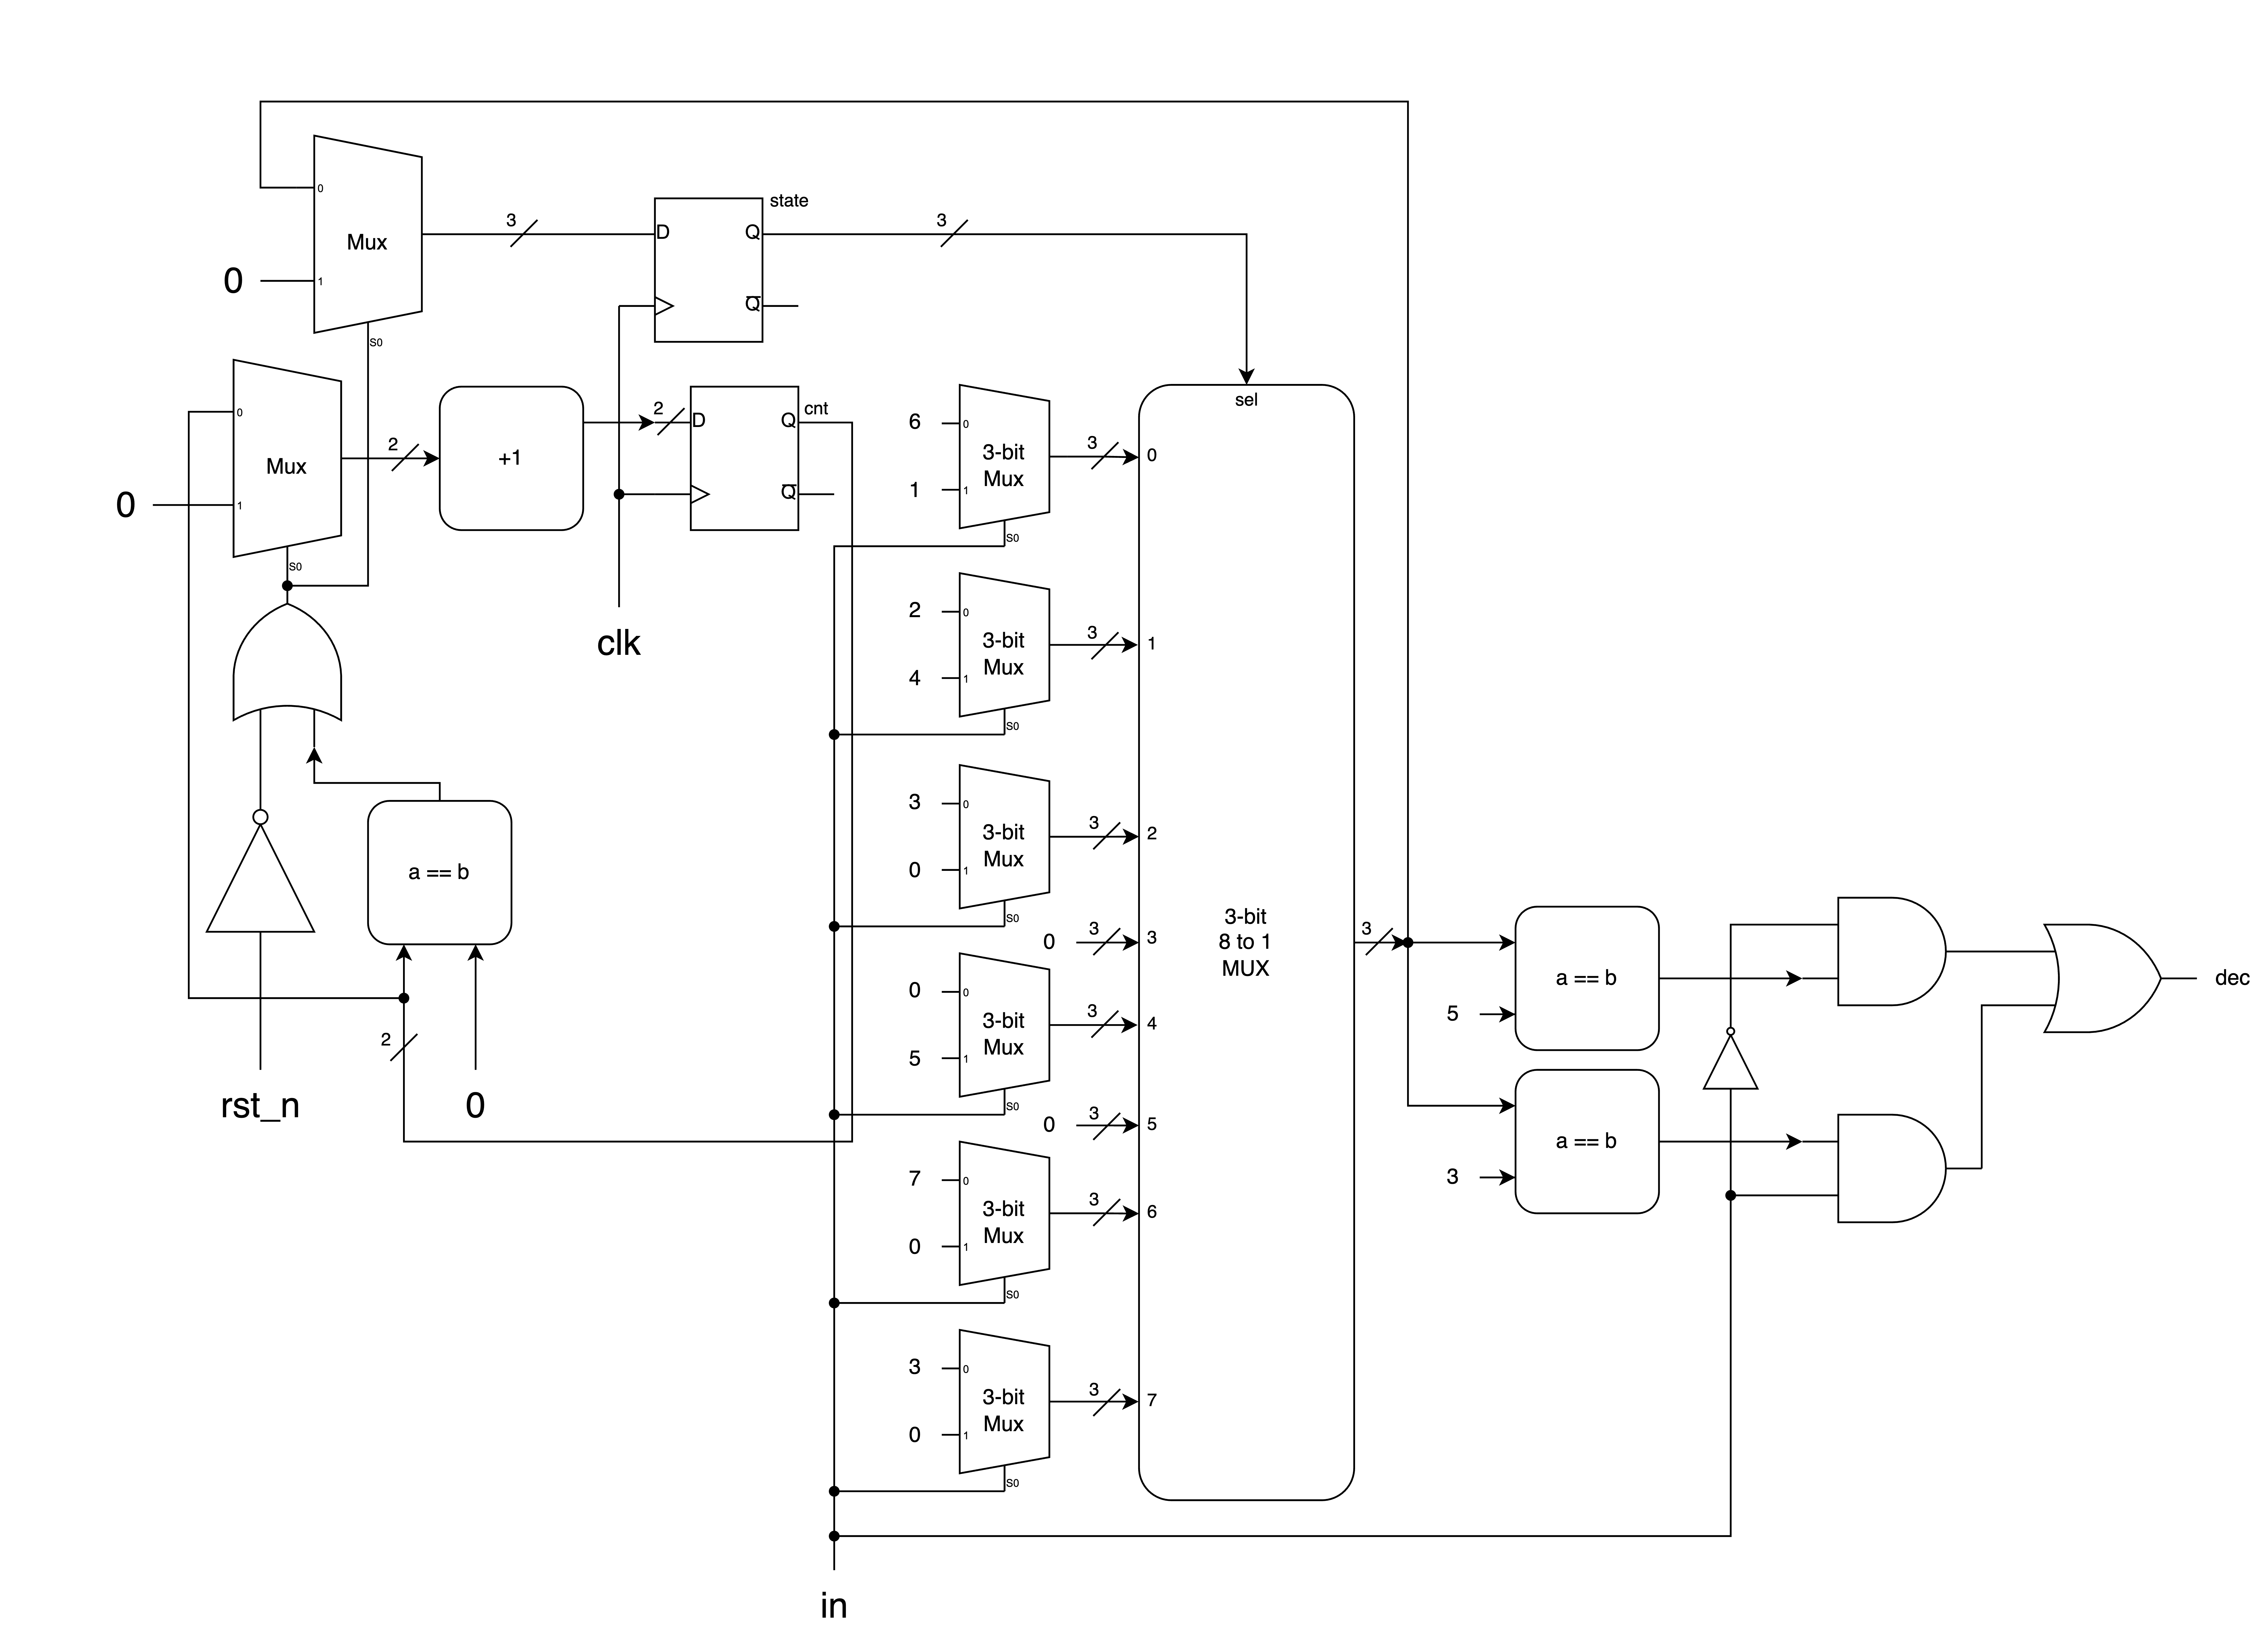
\includegraphics[width=\textwidth]{./img/Q4.png}
  \caption{Q4 Overall}
  \label{fig:Q4-Overall}
\end{figure}


\subsection{Testbench}

\begin{figure}[h!]
  \centering
  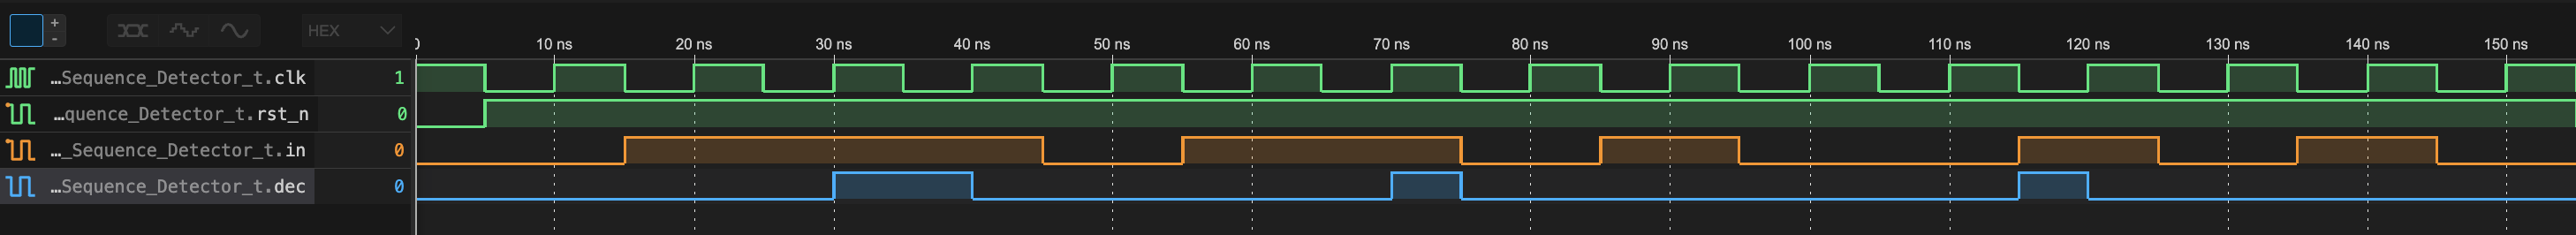
\includegraphics[width=\textwidth]{./img/Q4-tb.png}
  \caption{Q4 Testbench}
  \label{fig:Q4-tb}
\end{figure}

\section{FPGA: Implementation of advanced question 3}

最後的 FPGA 題需要將 Advanced Question 3 的 BIST 實作在 FPGA 上。\
透過開關控制 $scan\_en$ 以及 LFSR 的種子,\
並透過七段顯示器由左到右分別顯示出:$scan\_in, SDFF[7:4] (a), SDFF[3:0] (b), scan\_out$,\
以及使用 LED 顯示出 $SDFF[7], SDFF[6], \dots, SDFF[0]$。
\newpage
\subsection{Implement}

首先,因為 LFSR 的初始值會經 FPGA 上的 Switch 控制,因此我們修改了 SDFF,\
使其能夠接收一個 $rst\_d$ 的訊號來初始化。
\par
接著,由於需要讓人眼能更辨識並控制操作,題目規範了 LFSR 以及 SDFF 的操作必須由按鈕控制,\
按下後才能夠進行下一步操作。因此我們在 BIST, LFSR, Scan chain 都加上了一個 $d\_clk$ 的輸入訊號,\
只有當 $d\_clk = 1$ 的 clk posedge 才會改變狀態。\
按下按鈕後,訊號會先經過上次 Lab 提到的 debounce 以及 onepulse 電路,最後進到 BIST 中驅動狀態轉移。

\begin{figure}[h!]
  \centering
  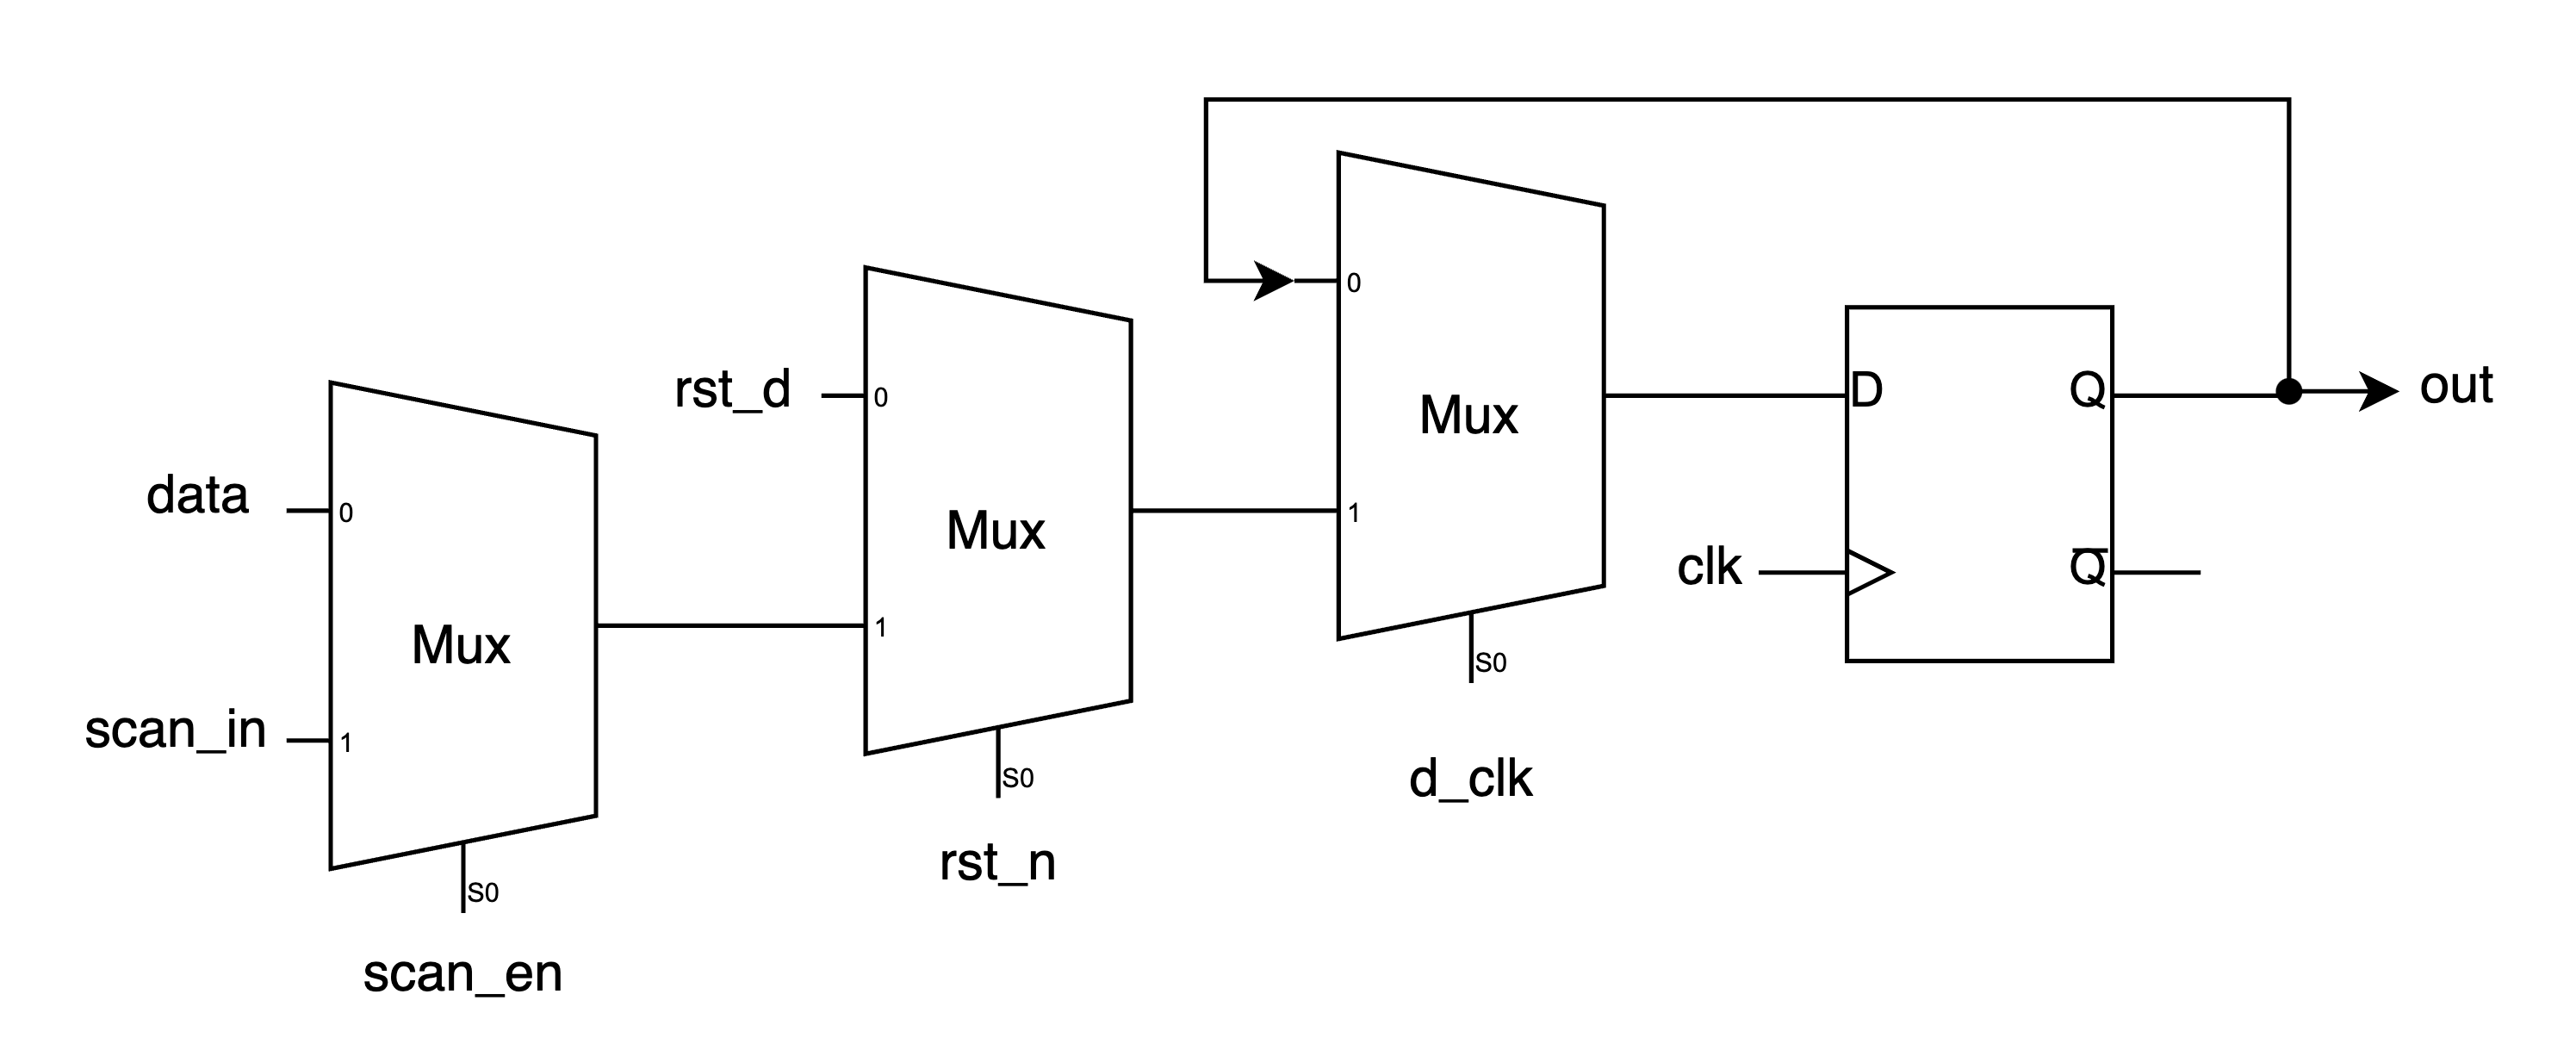
\includegraphics[width=\textwidth]{./img/FPGA-SDFF.png}
  \caption{FPGA SDFF}
  \label{fig:Q4-SDFF}
\end{figure}

\begin{figure}[h!]
  \centering
  
\includegraphics[width=\textwidth]{./img/FPGA-LFSR.png}
  \caption{FPGA LFSR}
  \label{fig:Q4-LFSR}
\end{figure}

\newpage

\begin{figure}[h!]
  \centering
  
\includegraphics[width=\textwidth]{./img/FPGA-SCD.png}
  \caption{FPGA Scan chain design}
  \label{fig:Q4-SCD}
\end{figure}

\begin{figure}[h!]
  \centering
  
\includegraphics[width=0.7\textwidth]{./img/FPGA-BIST.png}
  \caption{FPGA BIST}
  \label{fig:Q4-BIST}
\end{figure}

\section{Other}

\subsection{What we have learned}
\begin{itemize}
  \item 偽隨機產生器:隨機產生器的實現方式有很多種,以偽隨機產生器來說,mt19937 是一個非常可靠的例子,\
  但是其實現方式較為複雜,因此在一些簡單的情境中,LFSR 就是一個很適合的選擇。透過硬體電路的方式來產生偽隨機序列,\
  有時也會比軟體來得可靠,至少不會受到軟體環境,如 vivado 的影響而產生當機等狀況。
  \item CAM: 目前電腦系統中,比較主流的儲存方式是 RAM,但是如果要進行資料搜尋,在未排序的情況下,\
  就需要 $\mathcal{O}(n)$ 的時間複雜度來實現比較。而 CAM 由於其每個單元都有自己的比較器,\
  因此可以實現在 $\mathcal{O}(n)$ 的時間複雜度之下,找到對應的資料。雖然其硬體成本較高,\
  不適合用在通用型的裝置當中,但是在網路裝置如路由器中,由於需要快速的查找路由表,\
  因此 CAM 就會是一個很好的選擇。
  \item Moore vs Mealy machine: 在這次 Lab 中,我們實作了兩種的 Finite State Machine,\
  Moore machine 的輸出只跟狀態有關,而 Mealy machine 的輸出則是跟輸入以及狀態有關。\
  用時脈的角度來觀察,Moore 的輸出會類似於 Sequential Circuit,每個時脈週期只會改變一次輸出,\
  而 Mealy 因為輸入會直接影響輸出,因此具備 Combinational Circuit 的特性,只要輸入改變,輸出就會馬上改變。\
  這點在程式碼上也能看出明顯的差異,Moore 的輸出只需要在判下一個狀態時一起判斷即可,\
  但 Mealy 就需要額外拉一條線出來判斷輸出。       
\end{itemize}

\subsection{分工}
\begin{itemize}
  \item 陳克盈:Q2, Q3, FPGA
  \item 蔡明妡:Q1, Q4
\end{itemize}

\end{document}


